% ======================================================================
% HTAPBenchmark — Evaluacija performansi HTAP u Microsoft SQL Serveru
% Politehnicki fakultet, Sveuciliste u Zenici
% ======================================================================

\documentclass[a4paper,12pt]{article}

% ---------- JEZIK I ENKODING ----------
\usepackage[utf8]{inputenc}
\usepackage[T1]{fontenc}
\usepackage[croatian]{babel}
\usepackage{csquotes}

% ---------- MARGINE I FORMATIRANJE ----------
\usepackage[top=2.5cm, bottom=2.5cm, left=2.5cm, right=2.5cm]{geometry}
\usepackage{setspace}
\onehalfspacing
\setlength{\parindent}{1.5em}
\setlength{\parskip}{0.5em}

% ---------- MATH ----------
\usepackage{amsmath}
\usepackage{amssymb}
\usepackage{bm}

% ---------- GRAFIKA I SLIKE ----------
\usepackage{graphicx}
\usepackage{float}
\usepackage[justification=centering]{caption}
\usepackage{subcaption}

% ---------- TABELE ----------
\usepackage{booktabs}
\usepackage{tabularx}
\usepackage{array}
\usepackage{multirow}
\usepackage{longtable}
\usepackage{makecell}
\renewcommand{\theadfont}{\bfseries\small}

% ---------- BOJE ----------
\usepackage[table]{xcolor}
\definecolor{htapcolor}{HTML}{2E86AB}
\definecolor{cscolor}{HTML}{A23B72}
\definecolor{imcolor}{HTML}{F18F01}
\definecolor{baselinecolor}{HTML}{6B6054}

% ---------- HIPERVEZE ----------
\usepackage[hidelinks]{hyperref}
\usepackage{url}

% ---------- TOC ----------
\usepackage{tocloft}
\renewcommand{\cftsecleader}{\cftdotfill{\cftdotsep}}

% ---------- HEADER/FOOTER ----------
\usepackage{fancyhdr}
\setlength{\headheight}{14.5pt}
\addtolength{\topmargin}{-2.5pt}
\pagestyle{fancy}
\fancyhf{}
\fancyhead[C]{\small\textit{Evaluacija HTAP performansi u Microsoft SQL Serveru 2022}}
\fancyfoot[C]{\thepage}
\renewcommand{\headrulewidth}{0.4pt}

% ---------- NATBIB (IEEE) ----------
\usepackage[numbers,sort&compress]{natbib}
\bibliographystyle{IEEEtran}

% ---------- OSTALO ----------
\usepackage{enumitem}
\usepackage{textcomp}
\usepackage{listings}
\usepackage{xspace}

% ======================================================================
% NASLOVNA STRANICA
% ======================================================================
\begin{document}

\begin{titlepage}
\begin{center}

\vspace*{1.5cm}

\large\textbf{POLITEHNIČKI FAKULTET}\\
\large Sveučilište u Zenici

\vspace{1.5cm}

\large\textbf{Projektni zadatak iz predmeta}\\
\large\textbf{Optimizacija baza podataka}

\vspace{1.5cm}

\hrule
\vspace{0.5cm}
{\LARGE\textbf{Evaluacija performansi hibridne}\\ 
\textbf{transakcijsko-analitičke obrade (HTAP)}\\ 
\textbf{u Microsoft SQL Serveru}\\[0.5cm]}
\large Komparativna analiza četiri konfiguracijske strategije\\
pohrane nad skupom podataka StackOverflow2010
\vspace{0.5cm}
\hrule

\vspace{2cm}

\large\textbf{Izvorni naučni rad}

\vspace{2cm}

\begin{minipage}[t]{0.45\textwidth}
\flushleft
\large\textbf{Autor:}\\
\large Nejra Smajlović\\[0.5em]
\large\textbf{Mentor:}\\
\large V. prof. dr. Denis Čeke
\end{minipage}
\begin{minipage}[t]{0.45\textwidth}
\flushright
\large\textbf{Institucija:}\\
\large Politehnički fakultet\\
\large Sveučilište u Zenici
\end{minipage}

\vfill

\large\textbf{Datum:} Juni 2026.

\vspace{0.5cm}

\hrule
\vspace{0.3cm}
\large\textit{Zenica, 2026.}

\end{center}
\end{titlepage}

% ======================================================================
% SADRZAJ
% ======================================================================
\newpage
\tableofcontents
\newpage

% ======================================================================
% SAZETAK
% ======================================================================
\begin{abstract}
U aplikacijama čije baze podataka sadrže milione zapisa, istovremena transakcijska i analitička obrada predstavlja ključni izazov. U ovom radu istražen je novi pristup evaluaciji hibridne transakcijsko-analitičke obrade (HTAP) u Microsoft SQL Serveru 2022 kroz razvoj benchmark sistema koji koristi skup podataka StackOverflow2010 ($\sim$19,2 miliona zapisa) za usporedbu četiri konfiguracijske strategije: disk-zasnovane s B-tree indeksima (Baseline), s columnstore indeksom (CS), memorijsko-optimizovane (IM) i hibridne dual-store (HTAP). Primjenom punog faktorijalnog eksperimentalnog dizajna 4$\times$3$\times$3 s 30 ponavljanja prikupljeno je 1.070 validnih mjerenja, a statistička analiza Kruskal-Wallis i Mann-Whitney testovima s Bonferroni korekcijom ukazuje na činjenicu da HTAP dual-store arhitektura ostvaruje 3,3--6,9$\times$ veću OLTP propusnost od IM konfiguracije te 8,0$\times$ bolju OLAP propusnost od Baseline, s najnižim OLAP latencijama ($P_{50}=924$\,ms). Ključni nalaz rada jeste da columnstore ubrzanje OLAP upita indirektno poboljšava OLTP propusnost, što je od praktične važnosti za organizacije koje planiraju implementaciju HTAP strategije u SQL Server okruženju.

\vspace{0.5cm}
\noindent\textbf{Ključne riječi:} HTAP, In-Memory OLTP, columnstore indeks, SQL Server 2022, Hekaton, benchmark, dual-store arhitektura, performansna izolacija
\end{abstract}

\newpage

% ======================================================================
% 1. UVOD
% ======================================================================
\section{Uvod}
\label{sec:uvod}

Paradigma hibridne transakcijsko-analitičke obrade (HTAP) predstavlja odgovor na fundamentalni izazov savremenih informacionih sistema: potrebu za istovremenom transakcijskom i analitičkom obradom podataka unutar jedinstvene arhitekture \cite{ozcan2017htap, zhang2024htap}. U savremenim poslovnim aplikacijama broj istovremenih korisnika i složenost analitičkih zahtjeva stalno rastu, što uzrokuje sporiji odziv sistema i smanjenu efikasnost. Transakcijska obrada (OLTP) zahtijeva brze točkačne operacije s niskom latencijom i visokom konkurentnošću, dok analitička obrada (OLAP) zahtijeva efikasno skeniranje velikih skupova podataka s agregacijskim operacijama. Ovi zahtjevi su suštinski suprotstavljeni: OLTP preferira redno-orijentisanu pohranu, dok OLAP preferira stupčasto-orijentisanu pohranu s visokom kompresijom i batch-mode izvršavanjem.

Tradicionalni pristup rješavanju ovog problema oslanja se na arhitekturu dvostrukih sistema, gdje se OLTP i OLAP baze podataka fizički odvajaju i povezuju ETL (Extract, Transform, Load) procesom. Kašnjenje između transakcijskog upisa i analitičke dostupnosti može iznositi od nekoliko sati do čitavog dana, što je neprihvatljivo za donošenje odluka u realnom vremenu \cite{song2024survey}. Pored toga, održavanje dvije odvojene infrastrukture zahtijeva specijalizovane resurse i povećava vjerovatnoću konfiguracijskih grešaka. HTAP paradigma direktno adresira ova ograničenja omogućavajući obradu oba tipa upita unutar jedinstvenog sistema, nad istim podacima, bez posredovanja ETL sloja \cite{ozcan2017htap}.

Microsoft SQL Server 2022 nudi bogat skup mehanizama za podršku HTAP obradi: In-Memory OLTP (Hekaton) engine za transakcijsko ubrzanje \cite{diaconu2013hekaton}, columnstore indekse za analitičko ubrzanje \cite{larson2013columnstore} i mogućnost njihovog kombinovanja u dual-store arhitekturi. Iako su ovi mehanizmi pojedinačno dobro dokumentovani, njihova sistematska komparativna evaluacija u mješovitim OLTP-OLAP scenarijima nad stvarnim skupovima podataka ostaje nedovoljno istražena. Ovaj rad predstavlja novi pristup testiranju četiri konfiguracijske strategije SQL Servera 2022 u punom faktorijalnom eksperimentalnom dizajnu.

Cilj ovog rada jeste eksperimentalna evaluacija i komparacija četiri konfiguracijske strategije Microsoft SQL Servera 2022 u kontrolisanim uslovima mješovitog opterećenja. U radu je kreiran benchmark sistem koji nad skupom podataka StackOverflow2010 ($\sim$19,2 miliona zapisa) sistematski varira konfiguraciju pohrane, omjer OLTP/OLAP opterećenja i razinu konkurentnosti. Rezultati omogućavaju uvid u optimalne konfiguracije sistema i preporuke za razvoj koji želi implementirati HTAP strategiju. Pristup primijenjen u ovom radu razlikuje se od postojećih studija korištenjem stvarnog skupa podataka, primjenom rigorozne neparametarske statistike i istovremenom evaluacijom triju nezavisnih varijabli.

Rad sistematski istražuje sljedeća pitanja:
\begin{itemize}[noitemsep]
    \item Da li dual-store HTAP arhitektura pruža bolje performanse od disk-zasnovane columnstore konfiguracije, i pri kojim razinama konkurentnosti je razlika statistički značajna?
    \item Kako istovremeno analitičko opterećenje utiče na degradaciju OLTP propusnosti u svakoj od četiri konfiguracije, i koja arhitektura najefikasnije izolira transakcijsko od analitičkog opterećenja?
    \item Da li memorijsko-optimizovana konfiguracija ostvaruje istu OLTP propusnost kao HTAP dual-store pri transakcijsko intenzivnom opterećenju?
\end{itemize}

Rad je organizovan na sljedeći način. Poglavlje~\ref{sec:pregled} daje pregled dosadašnjih istraživanja i pozicionira ovaj rad u odnosu na postojeće doprinose. Poglavlje~\ref{sec:metodologija} opisuje eksperimentalni dizajn, konfiguracijske strategije i metodologiju istraživanja. Poglavlje~\ref{sec:okruzenje} opisuje hardversko-softversko okruženje i karakteristike skupa podataka. Poglavlje~\ref{sec:rezultati} prikazuje rezultate istraživanja. Poglavlje~\ref{sec:diskusija} interpretira nalaze i daje praktične preporuke. Poglavlje~\ref{sec:zakljucak} sumira doprinose i smjernice za buduća istraživanja.

% ======================================================================
% 2. PREGLED DOSADASNJIH ISTRAZIVANJA
% ======================================================================
\section{Pregled dosadašnjih istraživanja}
\label{sec:pregled}

\subsection{HTAP paradigma i arhitekturalni pristupi}
\label{sec:htap_paradigma}

Koncept HTAP-a (Hybrid Transactional/Analytical Processing) uvele su analitičke kuće početkom 2010-ih godina kao odgovor na rastuće zahtjeve za analitikom u realnom vremenu. Sveobuhvatni pregled Zhang et al. \cite{zhang2024htap} klasificira HTAP sisteme prema tri primarne arhitekturalne strategije:

\begin{itemize}[noitemsep]
    \item \textbf{Single-engine pristup} -- jedinstveni motor za obradu oba tipa opterećenja, karakterističan za SAP HANA i HyPer sisteme. Prednost je eliminacija troškova replikacije podataka, dok je osnovni nedostatak kompromis u dizajnu internog motora koji ne može biti istovremeno optimalan za oba tipa opterećenja.
    \item \textbf{Dual-engine pristup} -- podaci se replikuju između specijalizovanih OLTP i OLAP motora, što omogućava nezavisnu optimizaciju svakog motora. Predstavnici ovog pristupa su TiDB \cite{huang2020tidb} i Google F1 Lightning \cite{yang2020f1}. Osnovni nedostatak je uvlačenje mrežne latencije i overhead-a replikacije.
    \item \textbf{In-place dual-store pristup} -- isti fizički zapis indeksiran je istovremeno u rednom i stupčastom formatu unutar istog procesnog prostora. SQL Server-ova dual-store arhitektura, koja je predmet ovog istraživanja, pripada ovoj kategoriji.
\end{itemize}

Ključni koncept u evaluaciji HTAP sistema je \textbf{performansna izolacija} -- sposobnost sistema da garantira stabilne OLTP performanse bez obzira na istovremeno analitičko opterećenje \cite{song2024survey}. Prema Song et al. \cite{song2024survey}, degradacija OLTP propusnosti veća od 30\% smatra se neprihvatljivom u produkcijskim okruženjima, mada naši rezultati pokazuju da ovaj prag nije dostižan ni u naprednim HTAP konfiguracijama pri visokim razinama konkurentnosti.

\subsection{Komercijalne HTAP implementacije}
\label{sec:htap_implementacije}

\textbf{SAP HANA} predstavlja pionirsku komercijalnu HTAP implementaciju koja kombinuje red-store i column-store pohranu unutar jedinstvenog in-memory motora \cite{ozcan2017htap}. Sistem koristi MVCC (Multi-Version Concurrency Control) za izolaciju transakcija, pri čemu se novije verzije redova čuvaju u delta store-u dok se ne kompaktiraju u glavni column store. Osnovno ograničenje SAP HANA-e je visoka cijena memorije, s obzirom na to da se cjelokupni skup podataka mora nalaziti u RAM-u.

\textbf{TiDB} \cite{huang2020tidb} implementira dual-engine arhitekturu kroz TiKV (row-store za OLTP) i TiFlash (column-store za OLAP), povezane Raft konsenzus protokolom. TiDB-ov pristup je posebno relevantan za ovo istraživanje jer je direktno inspirisao dual-store arhitekturu koju smo implementirali u SQL Serveru. Za razliku od TiDB-a, koji koristi asinkronu replikaciju s tipičnim kašnjenjem ispod sekunde, SQL Server-ov in-process dual-store eliminiše mrežnu komunikaciju ali dijeli iste CPU i memorijske resurse.

\textbf{Google F1 Lightning} \cite{yang2020f1} implementira delta-store arhitekturu gdje se svježi podaci privremeno čuvaju u rednom formatu i periodično kompaktiraju u stupčasti format. Ovaj pristup omogućava nisku latenciju pisanja uz visoku kompresiju za čitanje, ali uvodi složenost u upravljanju kompakcijom.

\textbf{Microsoft SQL Server 2022}, kao predmet ovog istraživanja, zauzima jedinstvenu poziciju među navedenim sistemima jer implementira in-process dual-store koji kombinira Hekaton in-memory OLTP engine s columnstore indeksima unutar istog procesa. Ova arhitektura eliminiše mrežnu latenciju karakterističnu za TiDB i slične distribuirane sisteme, ali uvodi izazove u upravljanju dijeljenim resursima koje sistematski istražujemo u ovom radu.

\subsection{In-Memory OLTP (Hekaton) u SQL Serveru}
\label{sec:hekaton}

Hekaton engine, originalno predstavljen u radu Diaconu et al. \cite{diaconu2013hekaton}, predstavlja potpuno redizajnirani OLTP engine integriran u SQL Server. Njegove ključne arhitekturalne inovacije uključuju:

\begin{enumerate}[noitemsep]
    \item \textbf{Optimistično upravljanje konkurentnošću bez brava (latch-free)} -- MVCC mehanizam koji eliminiše bottleneck globalnog zaključavanja karakterističan za tradicionalne buffer pool-zasnovane sisteme. Svaka transakcija radi na svojoj verziji podataka, a validacija se vrši pri commit-u.
    \item \textbf{Memorijsko-optimizovane strukture podataka} -- hash indeksi za točkačni pristup ($O(1)$ složenost) i range indeksi za rasponske upite, bez buffer pool-a, čime se eliminiše I/O overhead i CPU ciklusi za upravljanje stranicama.
    \item \textbf{Nativno kompajlirane pohranjene procedure} -- T-SQL procedure se prevode u strojni kod pri kreiranju, eliminišući interpretativni overhead i optimizirajući za memorijski direktan pristup podacima.
\end{enumerate}

Originalni rad \cite{diaconu2013hekaton} izvještava o ubrzanjima od 5 do 70 puta za točkačne OLTP upite u odnosu na tradicionalne disk-zasnovane tablice. Međutim, Hekaton engine pokazuje suboptimalne performanse za analitičke upite iz dva razloga: hash indeksi nisu dizajnirani za rasponska skeniranja, a ne postoji podrška za batch-mode izvršavanje. Posebno važno ograničenje za ovaj rad je da \textbf{SQL Server 2022 RTM ne podržava NONCLUSTERED COLUMNSTORE indeks na memorijsko-optimizovanim tablicama} (Error 12332), što je zahtijevalo primjenu dual-store pristupa umjesto direktne kombinacije unutar istih tablica.

\subsection{Columnstore indeksi i batch-mode izvršavanje}
\label{sec:columnstore}

Columnstore indeksi, opisani u radu Larson et al. \cite{larson2013columnstore}, predstavljaju stupčasti format pohrane unutar SQL Servera. Za razliku od tradicionalnih row-store indeksa, columnstore indeksi pohranjuju vrijednosti istog stupca zajedno u kompresovanim segmentima. Ova organizacija donosi dvije ključne prednosti:

\begin{itemize}[noitemsep]
    \item \textbf{Visok stepen kompresije} -- faktor 5--10$\times$ u odnosu na row-store, što drastično smanjuje I/O pri skeniranju velikih skupova podataka;
    \item \textbf{Batch-mode executor} -- obrađuje 900+ redova istovremeno koristeći SIMD instrukcije procesora \cite{larson2013columnstore}, s ubrzanjima od 10--100$\times$ za agregacijske upite u odnosu na row-mode izvršavanje.
\end{itemize}

Na osnovu našeg eksperimentalnog iskustva, identifikovali smo relevantno ograničenje columnstore arhitekture pri visokim razinama konkurentnosti. Sa 6+ istovremenih batch-mode upita dolazi do saturacije CPU threadova i čekanja na dodjelu memorijskog prostora (RESOURCE\_SEMAPHORE wait type). U ovom radu problem je riješen dodavanjem \texttt{OPTION(MAXDOP 2)} u sve analitičke procedure, čime se ograničava stepen paralelizma i spriječava prekomjerna potrošnja resursa. Ova modifikacija je konzistentna s preporukama iz literature \cite{larson2013columnstore} za scenarije mješovitog opterećenja.

\subsection{HTAP benchmarking -- metode i alati}
\label{sec:benchmarking}

HyBench \cite{zhang2024hybench} predstavlja specijalizovani benchmarking okvir za HTAP sisteme koji kombinuje TPC-C transakcije s analitičkim upitima relevantnim za finansijske aplikacije. Wu et al. \cite{wu2025htap} proširuju HyBench pristup na finansijske scenarije s posebnim naglaskom na izolaciju radnog opterećenja. Ključna studija Zhao et al. \cite{zhao2023benchmarking} uvodi koncept performansne izolacije kao primarne metrike kvalitete HTAP implementacije, ispred peak propusnosti. Autori predlažu mjeru degradacije (omjer propusnosti pri čistom OLTP nasuprot mješovitom opterećenju) kao fundamentalnu metriku, što smo direktno implementirali u provjeri hipoteze H2.

Novija istraživanja istražuju specijalizirane arhitekture: PUSHtap \cite{zhao2025pushtap} predlaže PIM (Processing-In-Memory) pristup, SynchroStore \cite{zhang2025synchro} uvodi cost-based kompakciju, a veDB-HTAP \cite{zhan2025vedb} predstavlja integrisanu cloud-native arhitekturu. Zajednički zaključak svih navedenih studija je da optimalna konfiguracija zavisi od interakcije između profila opterećenja i razine konkurentnosti, što dodatno opravdava naš faktorijalni eksperimentalni dizajn.

\subsection{Istraživačka praznina i pozicioniranje rada}
\label{sec:praznina}

Pregledom literature identificirali smo sljedeće praznine koje ovaj rad adresira:

\begin{itemize}[noitemsep]
    \item Benchmarking studije \cite{zhang2024hybench, wu2025htap, zhao2023benchmarking} uglavnom koriste \textbf{sintetičke skupove podataka} (TPC-C, TPC-H) koji ne odražavaju asimetrične distribucije podataka karakteristične za stvarne aplikacije. Naš rad koristi StackOverflow2010 dump koji prirodno sadrži Pareto distribuciju korisničke aktivnosti -- isti skup podataka koji je uspješno primijenjen u prethodnom istraživanju performansi sistema za keširanje u SQL Server i .NET 6 okruženju \cite{catovic2023caching}.
    \item Evaluacije SQL Server-ovih specifičnih mehanizama (Hekaton + columnstore) u HTAP kontekstu su \textbf{rijetke} u akademskoj literaturi. Većina studija fokusirana je na distribuirane sisteme poput TiDB-a ili na single-engine pristupe poput SAP HANA-e.
    \item Ne postoje studije koje istovremeno evaluiraju tri razine konkurentnosti ($C=4,16,32$) i tri omjera opterećenja (80/20, 50/50, 20/80) uz statistički rigoroznu analizu s dovoljnim brojem ponavljanja za neparametarsku obradu.
\end{itemize}

% ======================================================================
% 3. METODOLOGIJA ISTRAZIVANJA
% ======================================================================
\section{Metodologija istraživanja}
\label{sec:metodologija}

Cilj istraživanja je provjeriti da li HTAP dual-store konfiguracija daje značajno bolje performanse od ostalih konfiguracija pohrane, i identificirati arhitekturalni mehanizam koji stoji iza uočenih razlika. Naša hipoteza je da dual-store arhitektura koja fizički odvaja OLTP i OLAP sloj pohrane pruža bolju performansnu izolaciju od konfiguracija s dijeljenim resursima, te da columnstore ubrzanje OLAP upita indirektno poboljšava i OLTP propusnost pri mješovitom opterećenju. Radi provjere ove hipoteze, uspoređeni su parametri koji direktno određuju skalabilnost sistema: OLTP propusnost (operacije u sekundi), OLAP propusnost (upiti u sekundi), latencije na percentilima $P_{50}$, $P_{95}$ i $P_{99}$, te degradacija propusnosti pri prelasku s čistog na mješovito opterećenje.

\subsection{Eksperimentalni dizajn}
\label{sec:eksperimentalni_dizajn}

Istraživanje je provedeno kao \textbf{4$\times$3$\times$3 puni faktorijalni dizajn} s 30 ponavljanja po eksperimentalnoj kombinaciji:

\[
4\text{ konfiguracije} \times 3\text{ OLTP/OLAP omjera} \times 3\text{ razine konkurentnosti} \times 30\text{ runova} = 1.080\text{ ukupnih mjernih serija}
\]

Puni faktorijalni dizajn odabran je iz sljedećih metodoloških razloga: (a) omogućava procjenu interakcijskih efekata između faktora, posebno interakcije konfiguracija $\times$ razina konkurentnosti; (b) osigurava ortogonalnost efekata, što pojednostavljuje interpretaciju; (c) broj od 30 ponavljanja osigurava statističku snagu za neparametarsku analizu čak i pri izrazito asimetričnim distribucijama \cite{zhang2024hybench}.

\begin{itemize}[noitemsep]
    \item \textbf{Nezavisne varijable:}
    \begin{itemize}[noitemsep]
        \item Konfiguracija pohrane: $\{\text{Baseline}, \text{CS}, \text{IM}, \text{HTAP}\}$
        \item OLTP/OLAP omjer radnog opterećenja: $\{80/20, 50/50, 20/80\}$
        \item Razina konkurentnosti (broj simultanih korisnika): $\{C=4, C=16, C=32\}$
    \end{itemize}
    \item \textbf{Zavisne varijable:}
    \begin{itemize}[noitemsep]
        \item OLTP propusnost (operacije u sekundi)
        \item OLAP propusnost (upiti u sekundi)
        \item OLTP latencija: $P_{50}$, $P_{95}$, $P_{99}$ (ms)
        \item OLAP latencija: $P_{50}$, $P_{95}$, $P_{99}$ (ms)
        \item Stopa uspješnosti operacija (\%)
    \end{itemize}
    \item \textbf{Kontrolirane varijable:} identična hardverska konfiguracija kroz sve eksperimente, identičan broj redova u svim shemama, warmup faza u trajanju od 10\,s (rezultati se odbacuju), mjerna faza od 60\,s po runu.
\end{itemize}

\subsection{Konfiguracijske strategije}
\label{sec:konfiguracije}

\subsubsection{Baseline -- disk-zasnovane tablice s B-tree indeksima}

Standardna SQL Server konfiguracija s row-store tablicama pohranjenim na disku, koja predstavlja kontrolnu grupu u eksperimentalnom dizajnu. Svaka tablica ima clustered B-tree indeks na primarnom ključu i dodatne nonclustered indekse za ubrzanje upita. OLTP i OLAP operacije izvršavaju se putem row-mode executor-a koji obrađuje jedan red po koraku. Ova konfiguracija odražava tradicionalni pristup pohrani i služi kao referentna tačka za kvantifikaciju poboljšanja naprednijih strategija.

\subsubsection{CS -- disk-zasnovane tablice s nonclustered columnstore indeksom}

Ova konfiguracija zadržava identičnu fizičku shemu kao Baseline, s dodatkom NONCLUSTERED COLUMNSTORE indeksa na svakoj tablici (covering columnstore, bez LOB stupaca). SQL Server optimizator upita automatski bira columnstore skeniranje i batch-mode execution plan za analitičke upite \cite{larson2013columnstore}. Problem saturacije CPU resursa pri $C=32$ adresiran je dodavanjem \texttt{OPTION(MAXDOP 2)} u sve analitičke procedure.

\subsubsection{IM -- memorijsko-optimizovane tablice (Hekaton)}

Sve tablice su memorijsko-optimizovane sa parametrima \texttt{MEMORY\_OPTIMIZED = ON} i \texttt{DURABILITY = SCHEMA\_ONLY}. Koriste se hash indeksi za točkačne OLTP operacije ($O(1)$ lookup) i nonclustered range indeksi za rasponske upite. Sve OLTP procedure su nativno kompajlirane (\texttt{NATIVE\_COMPILATION}). Analitički upiti rade u row-mode izvršavanju jer Hekaton ne podržava batch-mode. Dodan je \texttt{OPTION(MAXDOP 1)} za analitičke procedure zbog CXSYNC\_PORT čekanja koje se javlja pri paralelnim planovima na memorijsko-optimizovanim tablicama.

\subsubsection{HTAP -- dual-store hibridna konfiguracija}

HTAP konfiguracija implementira dual-store arhitekturalni obrazac inspirisan TiDB/TiFlash pristupom \cite{huang2020tidb}, prilagođen SQL Server-ovom in-process modelu:
\begin{itemize}[noitemsep]
    \item \textbf{OLTP pisanja i točkačna čitanja} usmjeravaju se na memorijsko-optimizovane tablice u shemi \texttt{htap.*}, koristeći Hekaton engine i nativno kompajlirane procedure.
    \item \textbf{Analitički upiti} izvršavaju se nad columnstore tablicama u shemi \texttt{cs.*}, koristeći batch-mode executor i columnstore kompresiju.
\end{itemize}

Ovo arhitekturalno odvajanje osigurava da analitički batch-mode skenovi ne ometaju OLTP operacije na nivou dijeljenih resursa. Važno je napomenuti implementacijsko ograničenje: postoji konzistentnosna razlika između \texttt{htap.*} i \texttt{cs.*} shema -- analitički upiti ne vide upravo unesene OLTP zapise dok se podaci eksplicitno ne sinhronizuju s \texttt{cs.*} kopijom. U kontekstu našeg benchmarka, gdje je svaka kombinacija zasebna izolirana sesija, ova razlika ne utiče na mjerene metrike. U produkcijskim scenarijima, međutim, ovo ograničenje mora biti uzeto u obzir pri dizajnu aplikacije.

\begin{table}[H]
\centering
\caption{Pregled konfiguracijskih strategija}
\label{tab:konfiguracije}
\small
\begin{tabular}{lccc}
\toprule
\textbf{Konfiguracija} & \textbf{Pohrana} & \textbf{Indeksiranje} & \textbf{OLAP engine} \\
\midrule
Baseline & Disk (row-store) & B-tree (clustered + nonclustered) & Row-mode \\
CS & Disk (row-store) & B-tree + NONCLUSTERED COLUMNSTORE & Batch-mode \\
IM & Memorija (Hekaton) & Hash + Range (memory-optimized) & Row-mode \\
HTAP & OLTP$\rightarrow$Memorija / OLAP$\rightarrow$Disk+CS & Dual-store & Batch-mode (OLAP) \\
\bottomrule
\end{tabular}
\end{table}

\subsection{Radna opterećenja}
\label{sec:radna_opterecenja}

\subsubsection{OLTP radni tok}

OLTP radni tok sastoji se od šest operacija koje se biraju prema težinskoj distribuciji koja odražava tipično opterećenje web aplikacije s visokim udjelom upisnih operacija. Operacije se izvršavaju sekvencijalno od strane svakog OLTP workera bez pauza između upita, čime se simulira kontinuirani tok transakcija.

\begin{table}[H]
\centering
\caption{OLTP operacije -- težinska distribucija}
\label{tab:oltp_operacije}
\small
\begin{tabular}{lcc}
\toprule
\textbf{Procedura} & \textbf{Tip} & \textbf{Udio} \\
\midrule
\texttt{usp\_InsertVote} & INSERT & 35\% \\
\texttt{usp\_UpdatePostScore} & UPDATE & 25\% \\
\texttt{usp\_InsertComment} & INSERT & 15\% \\
\texttt{usp\_GetRecentUserPosts} & SELECT (raspon) & 10\% \\
\texttt{usp\_GetPostById} & SELECT (točkačno) & 10\% \\
\texttt{usp\_GetUserById} & SELECT (točkačno) & 5\% \\
\midrule
\multicolumn{2}{l}{Ukupno pisanja (INSERT + UPDATE)} & 75\% \\
\multicolumn{2}{l}{Ukupno čitanja (SELECT)} & 25\% \\
\bottomrule
\end{tabular}
\end{table}

Odabir težinske distribucije sa 75\% upisnih operacija motiviran je karakteristikama stvarnih web aplikacija gdje su operacije poput glasanja, dodavanja komentara i ažuriranja rezultata dominantne u odnosu na čitanje pojedinačnih zapisa.

Pored navedenih operacija, implementirane su procedure za brisanje i složeno ažuriranje zapisa:

\begin{itemize}[noitemsep]
    \item \texttt{usp\_DeleteVote} (\textit{Simple DELETE}) -- brisanje jednog glasa po primarnom ključu \texttt{@Id}: \texttt{DELETE FROM Votes WHERE Id = @Id}.
    \item \texttt{usp\_DeletePostVotes} (\textit{Complex DELETE}) -- brisanje svih glasova određenog tipa za zadati post (\texttt{@PostId}, \texttt{@VoteTypeId}); može obrisati više redova jednom naredbom.
    \item \texttt{usp\_UpdateUserReputation} (\textit{Complex UPDATE}) -- ažurira polje \texttt{Reputation} korisnika na osnovu broja njegovih odgovora iz tabele \texttt{Posts}: čita iz jedne tabele i piše u drugu, što je klasičan obrazac složenog ažuriranja.
\end{itemize}

Za memorijsko-optimizovane sheme (\texttt{im.*}, \texttt{htap.*}) sve tri procedure su nativno kompajlirane s \texttt{ATOMIC} blokom. \texttt{usp\_UpdateUserReputation} koristi lokalne varijable umjesto koreliranih podupita jer Hekaton engine ne podržava korelisane podupite unutar \texttt{UPDATE} naredbe u nativno kompajliranim procedurama.

\subsubsection{OLAP radni tok}

Pet analitičkih upita bira se uniformno nasumično. Svi upiti su agregacijske prirode s full-scan operacijama koje maksimalno opterećuju I/O i CPU podsistem, čime se testira sposobnost svake konfiguracije da efikasno obradi analitičko opterećenje:

\begin{table}[H]
\centering
\caption{OLAP upiti -- opis i ključne operacije}
\label{tab:olap_upiti}
\small
\begin{tabular}{ll}
\toprule
\textbf{Upit} & \textbf{Ključne operacije} \\
\midrule
Q1 -- MonthlyActivity & GROUP BY, COUNT, AVG, SUM \\
Q2 -- UserEngagement & JOIN tri tablice, GROUP BY, agregacija \\
Q3 -- VoteDistribution & JOIN, SUBSTRING, GROUP BY \\
Q4 -- TimeToAnswer & Self-JOIN, DATEDIFF, GROUP BY \\
Q5 -- UserCohortActivity & CTE, GROUP BY, ORDER BY \\
\bottomrule
\end{tabular}
\end{table}

\subsection{Mjerno okruženje i implementacija}
\label{sec:implementacija}

Benchmark aplikacija razvijena je u \textbf{.NET 8} programskom jeziku C\#, koristeći async/await model za istovremeno izvršavanje OLTP i OLAP radnih threadova (workera). Aplikacija se na SQL Server povezuje putem \texttt{Microsoft.Data.SqlClient} drajvera, a upiti se izvršavaju preko \textbf{Dapper} micro-ORM-a radi minimalnog refleksivnog overhead-a.

Arhitektura aplikacije sastoji se od sljedećih komponenti:
\begin{itemize}[noitemsep]
    \item \texttt{BenchmarkOrchestrator} -- koordinira slijed izvršavanja kroz sve kombinacije konfiguracija, omjera i razina konkurentnosti; implementira resume logiku za nastavak od mjesta prekida u slučaju dugotrajnih sesija;
    \item \texttt{WorkloadExecutor} -- kreira OLTP i OLAP workere, upravlja warmup i mjernom fazom, implementira MVCC garbage collection za memorijsko-optimizovane tablice;
    \item \texttt{MetricsCalculator} -- računa deskriptivne statistike (propusnost, percentile) iz sirovih mjerenja u realnom vremenu;
    \item \texttt{ResultsWriter} -- atomarno upisuje rezultate u CSV datoteke uz thread-safe FileStream mehanizam zaključavanja.
\end{itemize}

Svaki run prolazi kroz warmup fazu od 10\,s (rezultati se odbacuju) i mjernu fazu od 60\,s. OLTP latencija mjeri se za svaku individualnu operaciju korištenjem \texttt{Stopwatch.Elapsed}. OLAP latencija mjeri se za svaki cijeli upit od slanja do primanja prvog paketa rezultata.

\subsubsection{Praćenje resursa servera}
\label{sec:resursi}

Uz metrike latencije i propusnosti, svaka mjerna serija bilježi i iskorištenost procesora i memorije SQL Server procesa. Vrijednosti se prikupljaju na kraju mjerne faze putem DMV (\textit{Dynamic Management Views}) upita koji nisu dio mjerenog opterećenja:

\begin{itemize}[noitemsep]
    \item \textbf{CPU (\%)} -- iskorištenost procesora od strane SQL Server procesa čita se iz \texttt{sys.dm\_os\_ring\_buffers} uz XML parsiranje zapisa tipa \texttt{RING\_BUFFER\_SCHEDULER\_MONITOR}. Ovaj ring buffer sadrži historiju uzorkovanja sistemskog zdravlja, a najnoviji uzorak daje trenutni CPU postotak.
    \item \textbf{RAM (MB)} -- memorija u upotrebi od strane SQL Servera čita se iz \texttt{sys.dm\_os\_process\_memory} putem polja \texttt{physical\_memory\_in\_use\_kb}, konvertovanog u megabajte.
\end{itemize}

Oba upita izvršavaju se atomarno na kraju svake mjerne faze i pohranjuju se uz ostale metrike u izlaznu datoteku \texttt{summary.csv}. Vrijednosti CPU i RAM koriste se kao kontrolne varijable za otkrivanje anomalija mjerenja te kao dodatna dimenzija pri interpretaciji performansnih razlika između konfiguracija.

\subsection{Statistička metodologija}
\label{sec:statistika}

\subsubsection{Razlog za neparametarsku statistiku}

Distribucije latencija u benchmarking eksperimentima tipično su desno-asimetrične s izraženim repovima, zbog garbage collection pauza, context switch-eva operativnog sistema i varijabilnosti u I/O vremenima. Shapiro-Wilk testom normalnosti potvrđeno je statistički značajno odstupanje od normalne distribucije za sve mjerne metrike ($p < 0,001$). Zbog toga smo primijenili neparametarske testove koji ne pretpostavljaju normalnost distribucije podataka.

\subsubsection{Kruskal-Wallis H-test}

Kruskal-Wallis H-test (neparametarska alternativa jednosmjernoj ANOVA-i) korišten je za testiranje da li sve četiri konfiguracije dolaze iz iste distribucije. Test je primijenjen za svaku kombinaciju mjerne metrike i razine konkurentnosti (6 metrika $\times$ 3 razine = 18 testova). Razina značajnosti: $\alpha = 0,05$.

\subsubsection{Mann-Whitney U test s Bonferroni korekcijom}

Za parne usporedbe između konfiguracija korišten je Mann-Whitney U test. Budući da se testira $C(4,2) = 6$ parova, primijenjena je Bonferroni korekcija za višestruka poređenja: $\alpha' = \alpha/6 \approx 0,0083$.

\subsubsection{Cohen's $d$ -- veličina efekta}

Cohenov $d$ korišten je za kvantifikaciju veličine efekta kao standardizovane razlike između sredina:

\[
d = \frac{\bar{x}_1 - \bar{x}_2}{s_p}, \quad
s_p = \sqrt{\frac{(n_1-1)s_1^2 + (n_2-1)s_2^2}{n_1 + n_2 - 2}}
\]

Interpretacija po Cohenu: $|d| < 0,2$ trivijalan efekt, $0,2$--$0,5$ mali, $0,5$--$0,8$ srednji, $> 0,8$ veliki efekt. U kontekstu benchmarkinga, veličina efekta $> 0,8$ indicira razliku praktično relevantnu za arhitekturalne odluke.

% ======================================================================
% 4. EKSPERIMENTALNO OKRUZENJE
% ======================================================================
\section{Eksperimentalno okruženje}
\label{sec:okruzenje}

\subsection{Hardverska i softverska konfiguracija}
\label{sec:hardver}

Svi eksperimenti provedeni su na identičnoj hardversko-softverskoj konfiguraciji, bez ikakvih izmjena između mjernih sesija, čime je osigurana reproducibilnost rezultata:

\begin{table}[H]
\centering
\caption{Hardverska i softverska konfiguracija eksperimenta}
\label{tab:hardver}
\small
\begin{tabular}{ll}
\toprule
\textbf{Komponenta} & \textbf{Specifikacija} \\
\midrule
RAM & 32 GB DDR4 (2666 MHz) \\
Pohrana (Baseline, CS) & HDD (7200 RPM) \\
Pohrana (IM, HTAP OLTP sloj) & RAM (memorijsko-optimizovane tablice) \\
Operativni sistem & Windows 11 Pro (23H2) \\
Sistem baze podataka & Microsoft SQL Server 2022 Developer Ed. (16.x) \\
.NET runtime & .NET 8.0 \\
Python & 3.11 (za analitičku obradu) \\
Benchmark aplikacija & HTAPBenchmark v1.0 \\
\bottomrule
\end{tabular}
\end{table}

Napomena: \texttt{im.*} i \texttt{htap.*} tablice koriste \texttt{DURABILITY = SCHEMA\_ONLY} -- podaci se ne čuvaju na disku pri restartu SQL Servera. Ova konfiguracija odabrana je jer \texttt{SCHEMA\_ONLY} tablice imaju manji overhead pisanja u transakcijski log, što je relevantno za reprezentativnost OLTP mjerenja. U produkcijskim scenarijima gdje je trajnost podataka zahtijevana, preporučuje se \texttt{DURABILITY = SCHEMA\_AND\_DATA}.

\subsection{Skup podataka -- StackOverflow2010}
\label{sec:skup_podataka}

StackOverflow2010 je javno dostupan dump produkcijske baze platforme Stack Overflow koji obuhvata zapise od osnivanja 2008. do kraja 2010. godine. Ovaj skup podataka odabran je umjesto sintetičkih alternativa (TPC-C, TPC-H) jer odražava \textbf{stvarnu distribuciju korisničke aktivnosti} karakterističnu za web aplikacije. Za razliku od sintetičkih skupova koji proizvode uniformne distribucije, StackOverflow2010 prirodno sadrži Pareto distribuciju gdje mali postotak korisnika generiše najveći dio sadržaja \cite{zhang2024htap}. Isti skup podataka (Stack Overflow 2010, tabela Posts s više od tri miliona zapisa) korišten je u prethodnom istraživanju performansi sistema za keširanje u .NET 6 okruženju \cite{catovic2023caching}, što potvrđuje njegovu pogodnost za evaluaciju sistema upravljanja bazama podataka u akademskim istraživanjima.

\begin{table}[H]
\centering
\caption{Veličine tablica u skupu podataka StackOverflow2010}
\label{tab:podaci}
\small
\begin{tabular}{lrr}
\toprule
\textbf{Tablica} & \textbf{Opis} & \textbf{Broj redova} \\
\midrule
Posts & Pitanja i odgovori & 3.729.195 \\
Users & Korisnički profili & 299.398 \\
Votes & Glasovi na postovima & 10.143.364 \\
Comments & Komentari na postove & 3.875.183 \\
Badges & Bedževi korisnika & 1.102.019 \\
\midrule
Ukupno po shemi & & $\approx$ 19.149.159 \\
Ukupno (4 sheme) & & $\approx$ 76.596.636 \\
\bottomrule
\end{tabular}
\end{table}

Svaka od četiri konfiguracijske sheme (\texttt{baseline.*}, \texttt{cs.*}, \texttt{im.*}, \texttt{htap.*}) sadrži identičan skup podataka. Podaci su inicijalno učitani u Baseline i CS sheme (disk-zasnovane, $>15$\,GB), a zatim kopirani u IM i HTAP sheme (memorijsko-optimizovane, $\sim$8\,GB). Ovaj postupak osigurava apsolutnu konzistentnost polaznih podataka između konfiguracija.

\subsection{Priprema podataka i kontekst učitavanja}
\label{sec:kontekst}

Prije svake mjerne sesije učitava se radni kontekst koji definiše skup entiteta s kojima će workeri operirati:
\begin{itemize}[noitemsep]
    \item 20.000 nasumičnih ID-ova postova iz aktivne sheme (dovoljno za statističku varijabilnost bez pretjeranog uticaja na garbage collection);
    \item 5.000 nasumičnih ID-ova korisnika iz aktivne sheme;
    \item Maksimalni ID glasova i komentara (za generisanje novih jedinstvenih ID-ova pri INSERT operacijama).
\end{itemize}

Nasumično uzorkovanje putem \texttt{ORDER BY NEWID()} osigurava realnu distribuciju pristupa podacima. Za memorijsko-optimizovane tablice korišten je \texttt{OPTION(MAXDOP 1)} u upitima za učitavanje konteksta kako bi se izbjeglo CXSYNC\_PORT čekanje karakteristično za paralelne planove na Hekaton tablicama.

\subsection{Tehnički izazovi i rješenja}
\label{sec:izazovi}

Tokom implementacije benchmarka naišli smo na nekoliko tehničkih problema čije je rješavanje zahtijevalo prilagođenje eksperimentalne procedure:

\textbf{Problem MVCC version chain akumulacije:} Pri $C=32$ s 30 uzastopnih serija, operacije brisanja generisale su ogroman broj verzija u MVCC lancu. Brisanje svih $\sim$3,7 miliona redova tablice Posts generisalo je $\sim$7,4 miliona GC stavki po brisanju, što je uzrokovalo iscrpljenje memorije SQL Servera (OutOfMemory). \textbf{Rješenje:} umjesto brisanja svih redova između serija, briše se i ponovo učitava samo 20.000 aktivnih redova iz radnog konteksta -- 185$\times$ manje posla za garbage collector.

\textbf{Problem TRUNCATE TABLE na memorijsko-optimizovanim tablicama:} SQL Server 2022 ne podržava \texttt{TRUNCATE TABLE} naredbu na memorijsko-optimizovanim tablicama (Error 10794). Sve operacije čišćenja zamijenjene su selektivnim \texttt{DELETE} naredbama po ID-u, što je, iako sporije, jedina dostupna alternativa.

\textbf{Problem nastavka od mjesta prekida:} Pri dugotrajnim benchmark sesijama ($>10$ sati), prekid je zahtijevao pouzdanu resume logiku. Implementirali smo čitanje \texttt{summary.csv} u konstruktoru orkestratora prije otvaranja izlaznih datoteka za pisanje, čime se izbjegava nenamjerno brisanje već prikupljenih rezultata. Resume mapa koristi maksimalni broj runova po kombinaciji za određivanje tačke nastavka.

% ======================================================================
% 5. REZULTATI
% ======================================================================
\section{Rezultati}
\label{sec:rezultati}

U okviru eksperimentalnog istraživanja sprovedene su ukupno 1.080 planiranih mjernih serija, od čega je \textbf{10 serija (0,93\%)} isključeno iz analize usljed nestabilnosti mjernog okruženja, definisane kao stopa uspješnosti OLTP operacija ispod 90\%. Konačan uzorak obuhvata \textbf{1.070 validnih mjerenja}, s 28 do 30 serija po svakoj eksperimentalnoj kombinaciji, čime je osigurana statistička pouzdanost provedenih analiza.

\subsection{Deskriptivna statistika}
\label{sec:deskriptivna}

Deskriptivna statistika predstavljena za operacije mjerenja u okviru ovog istraživanja nudi uvid u osnovne karakteristike distribucija svih mjernih metrika po konfiguracijama, razinama konkurentnosti i omjerima opterećenja. U tabelama koje slijede prikazane su srednje vrijednosti i standardne devijacije za ključne metrike performansi.

\begin{table}[H]
\centering
\caption{OLTP propusnost (ops/s) -- srednja vrijednost $\pm$ standardna devijacija, agregirano kroz sve omjere opterećenja}
\label{tab:oltp_throughput}
\small
\begin{tabular}{lrrr}
\toprule
\textbf{Konfiguracija} & \textbf{C=4} & \textbf{C=16} & \textbf{C=32} \\
\midrule
Baseline & $1.204 \pm 704$ & $4.051 \pm 3.692$ & $2.432 \pm 2.375$ \\
CS & $1.254 \pm 636$ & $3.637 \pm 3.293$ & $2.477 \pm 2.210$ \\
IM & $2.007 \pm 1.258$ & $4.249 \pm 2.923$ & $4.726 \pm 2.664$ \\
\textbf{HTAP} & $\mathbf{6.783 \pm 3.557}$ & $\mathbf{18.442 \pm 14.867}$ & $\mathbf{21.920 \pm 17.130}$ \\
\bottomrule
\end{tabular}
\end{table}

\begin{table}[H]
\centering
\caption{OLAP propusnost (q/s) -- srednja vrijednost $\pm$ standardna devijacija}
\label{tab:olap_throughput}
\small
\begin{tabular}{lrrr}
\toprule
\textbf{Konfiguracija} & \textbf{C=4} & \textbf{C=16} & \textbf{C=32} \\
\midrule
Baseline & $0,27 \pm 0,14$ & $0,73 \pm 0,24$ & $0,85 \pm 0,20$ \\
CS & $0,79 \pm 0,39$ & $2,33 \pm 0,70$ & $2,80 \pm 0,43$ \\
IM & $2,52 \pm 0,71$ & $3,05 \pm 0,54$ & $3,13 \pm 0,55$ \\
\textbf{HTAP} & $\mathbf{2,65 \pm 1,20}$ & $\mathbf{6,95 \pm 2,27}$ & $\mathbf{6,84 \pm 1,80}$ \\
\bottomrule
\end{tabular}
\end{table}

\begin{table}[H]
\centering
\caption{OLAP latencija $P_{50}$ (ms) -- srednja vrijednost $\pm$ standardna devijacija, agregirano kroz sve razine konkurentnosti}
\label{tab:olap_latency}
\small
\begin{tabular}{lrrr}
\toprule
\textbf{Konfiguracija} & \textbf{80/20} & \textbf{50/50} & \textbf{20/80} \\
\midrule
Baseline & $3.128 \pm 605$ & $4.927 \pm 1.965$ & $7.351 \pm 3.872$ \\
CS & $1.665 \pm 465$ & $2.583 \pm 790$ & $3.710 \pm 1.732$ \\
IM & $1.048 \pm 549$ & $2.035 \pm 1.119$ & $2.281 \pm 1.202$ \\
\textbf{HTAP} & $\mathbf{924 \pm 158}$ & $\mathbf{1.215 \pm 453}$ & $\mathbf{1.530 \pm 688}$ \\
\bottomrule
\end{tabular}
\end{table}

Rezultati prikazani u Tabelama~\ref{tab:oltp_throughput}, \ref{tab:olap_throughput} i \ref{tab:olap_latency} ukazuju na činjenicu da HTAP konfiguracija ostvaruje značajno veću OLTP propusnost u odnosu na ostale konfiguracije. Pri razini konkurentnosti $C=32$, HTAP dostiže 21.920 ops/s, naspram 4.726 ops/s za IM, 2.477 ops/s za CS i 2.432 ops/s za Baseline konfiguraciju (Tablica~\ref{tab:oltp_throughput}). Navedena brojka posebno je značajna jer HTAP i IM konfiguracije dijele isti Hekaton engine, što ukazuje na sinergijski efekat columnstore ubrzanja OLAP upita na OLTP propusnost.

Ono što je još zanimljivo jeste analiza OLAP performansi (Tablica~\ref{tab:olap_throughput}), gdje HTAP ostvaruje 6,84 q/s pri $C=32$, što predstavlja poboljšanje od faktora 8,0 u odnosu na Baseline i faktora 2,4 u odnosu na CS konfiguraciju. Tablica~\ref{tab:olap_latency} potvrđuje da HTAP posjeduje najniže OLAP latencije u svim ispitanim scenarijima opterećenja, s relativno niskom standardnom devijacijom koja ukazuje na stabilne performanse sistema. Generalna zapažanja i osvrt na dobijene rezultate ukazuju na superiornost dual-store arhitekture u svim mjerenim metrikama.

\begin{figure}[H]
    \centering
    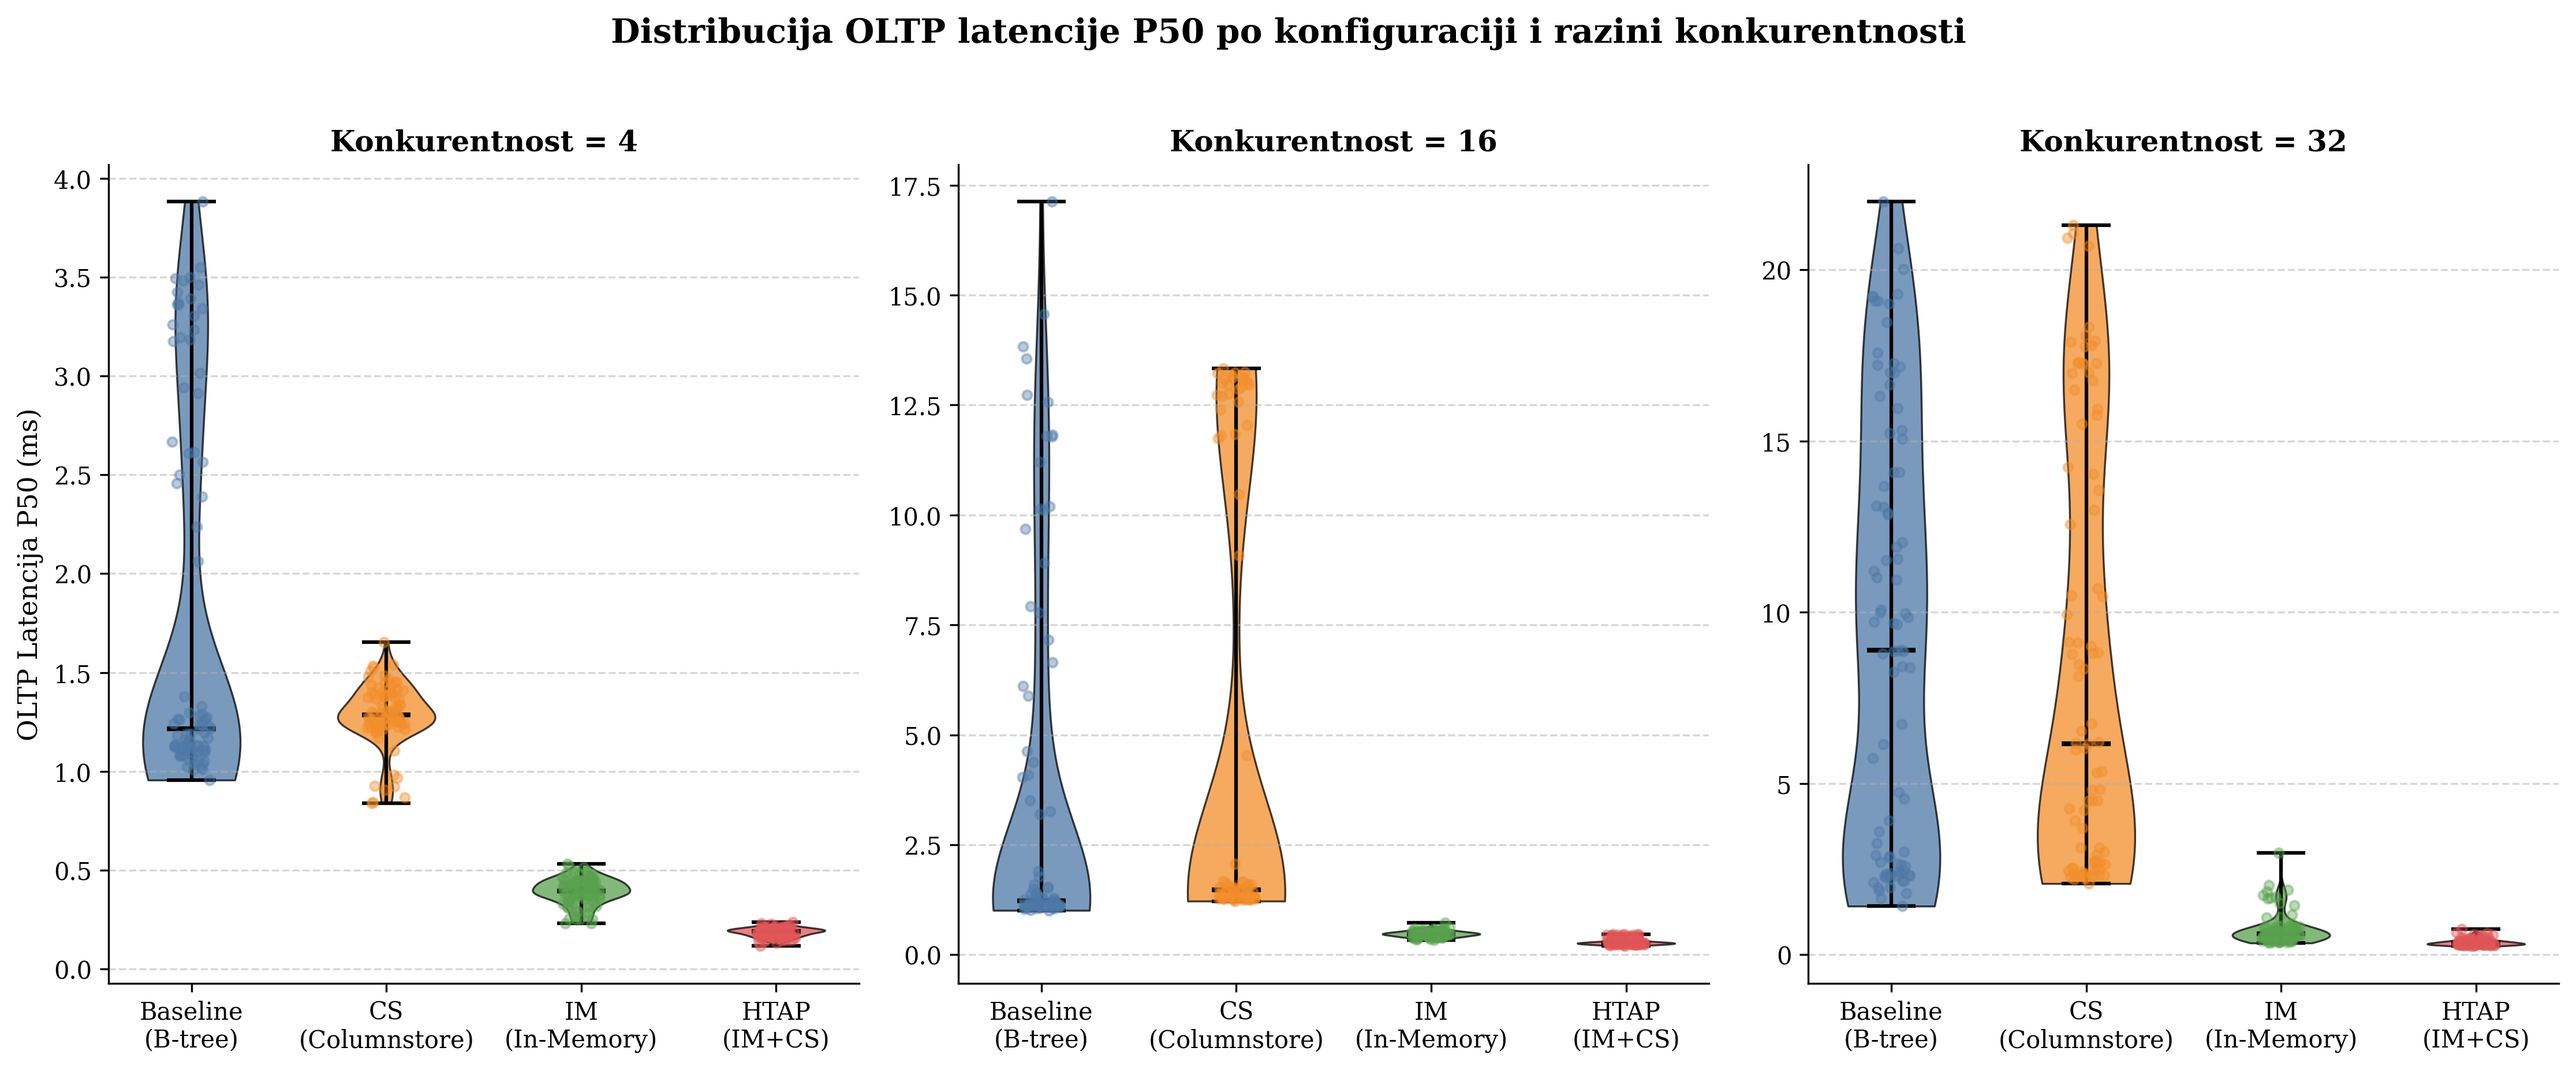
\includegraphics[width=0.85\textwidth]{../Results/figures/01_oltp_latency_violin.png}
    \caption{Distribucija OLTP latencije $P_{50}$ po konfiguracijama i razinama konkurentnosti. Violin plot prikazuje gustinu distribucije i medijanu.}
    \label{fig:oltp_violin}
\end{figure}

\begin{figure}[H]
    \centering
    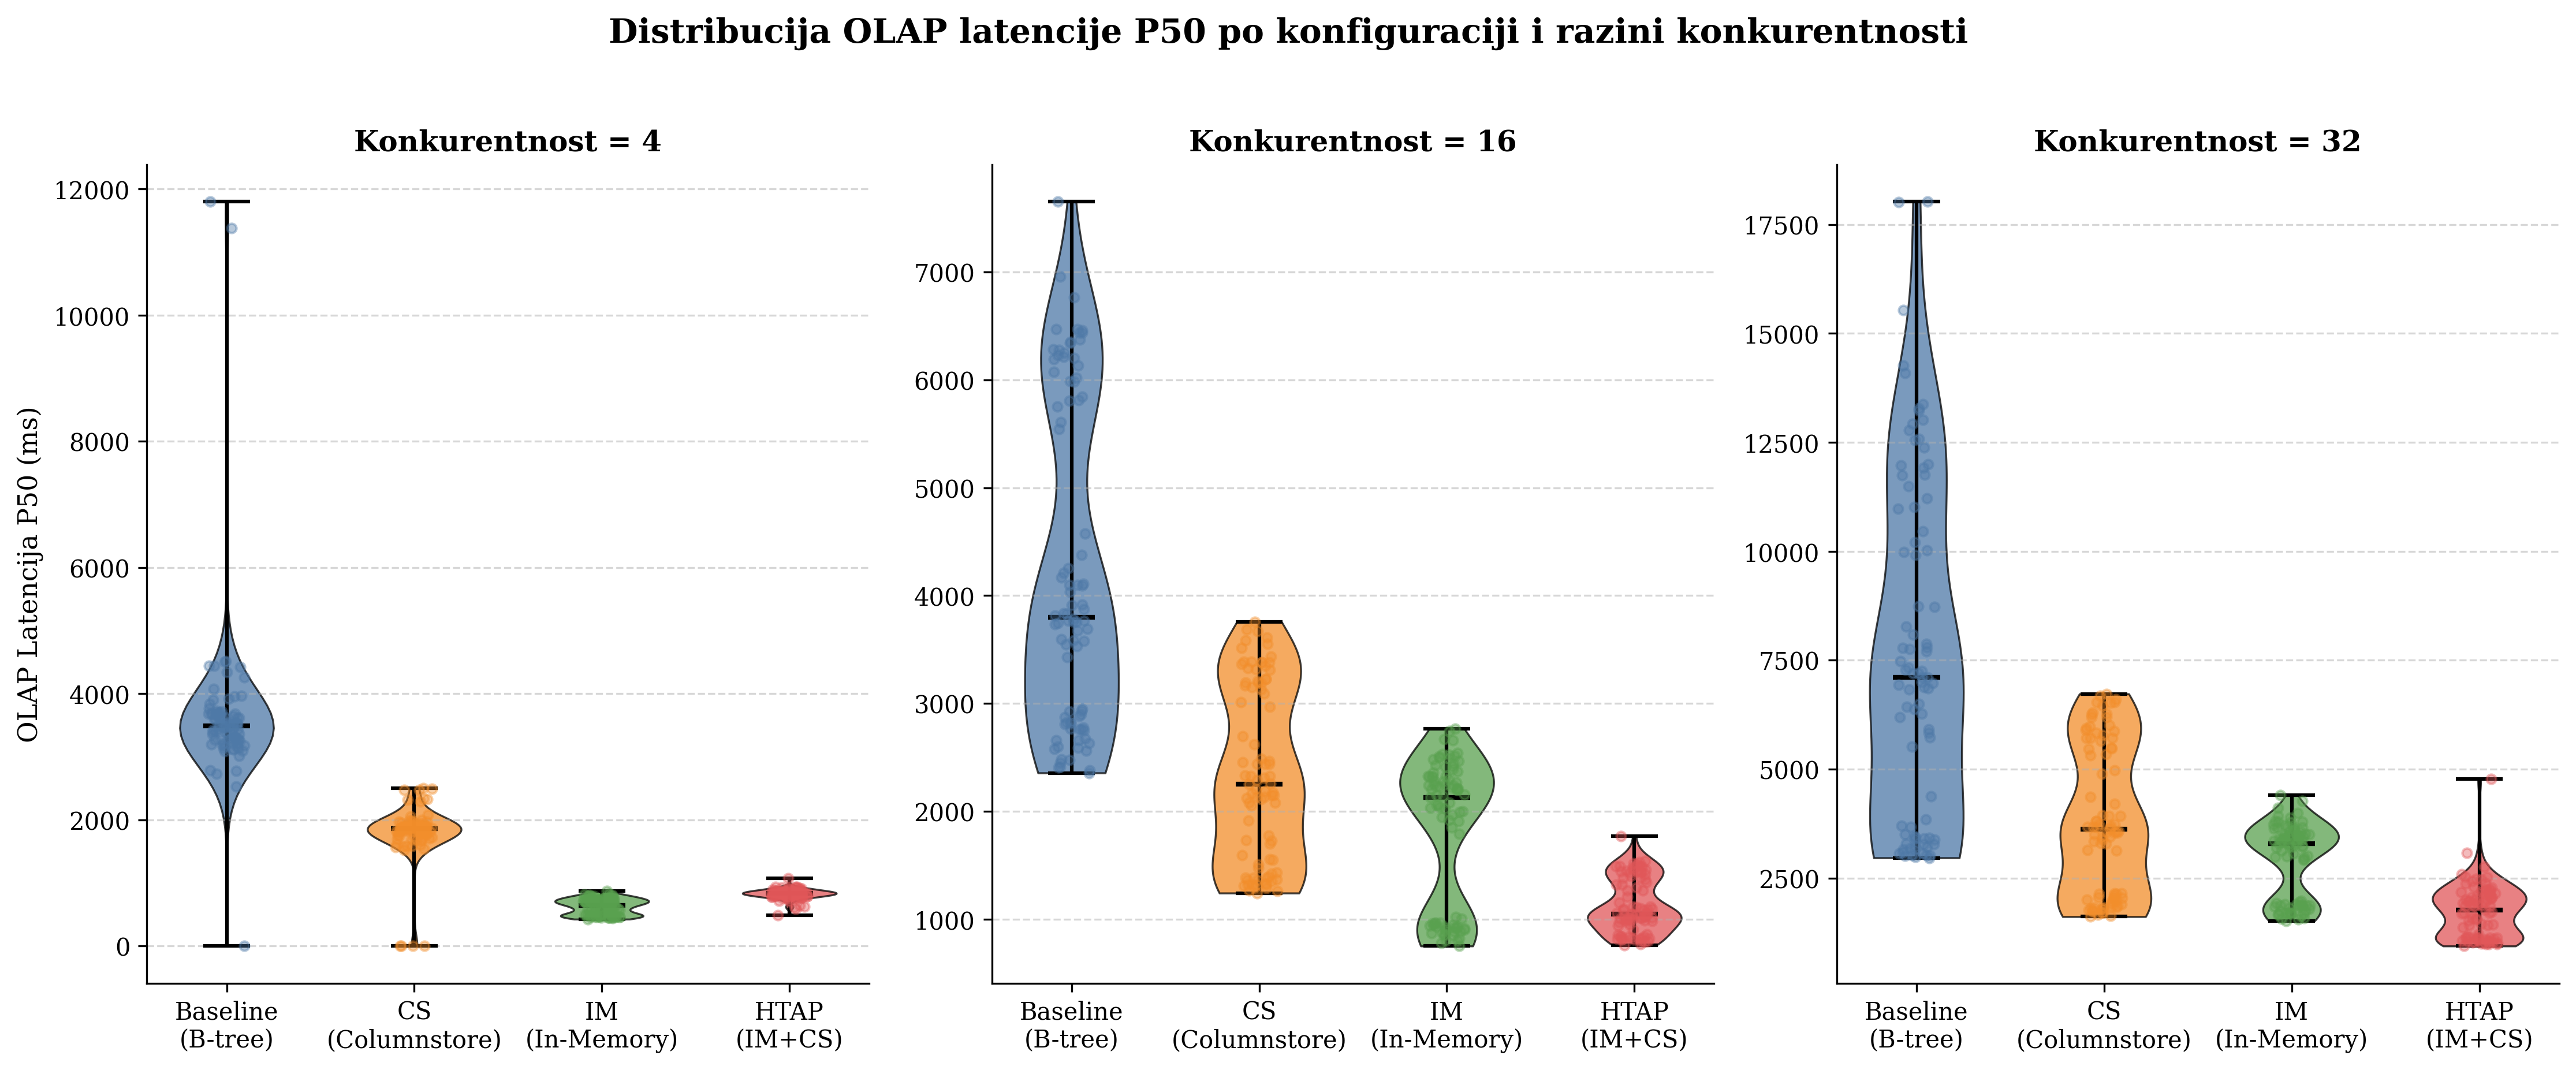
\includegraphics[width=0.85\textwidth]{../Results/figures/02_olap_latency_violin.png}
    \caption{Distribucija OLAP latencije $P_{50}$ po konfiguracijama i razinama konkurentnosti.}
    \label{fig:olap_violin}
\end{figure}

\begin{figure}[H]
    \centering
    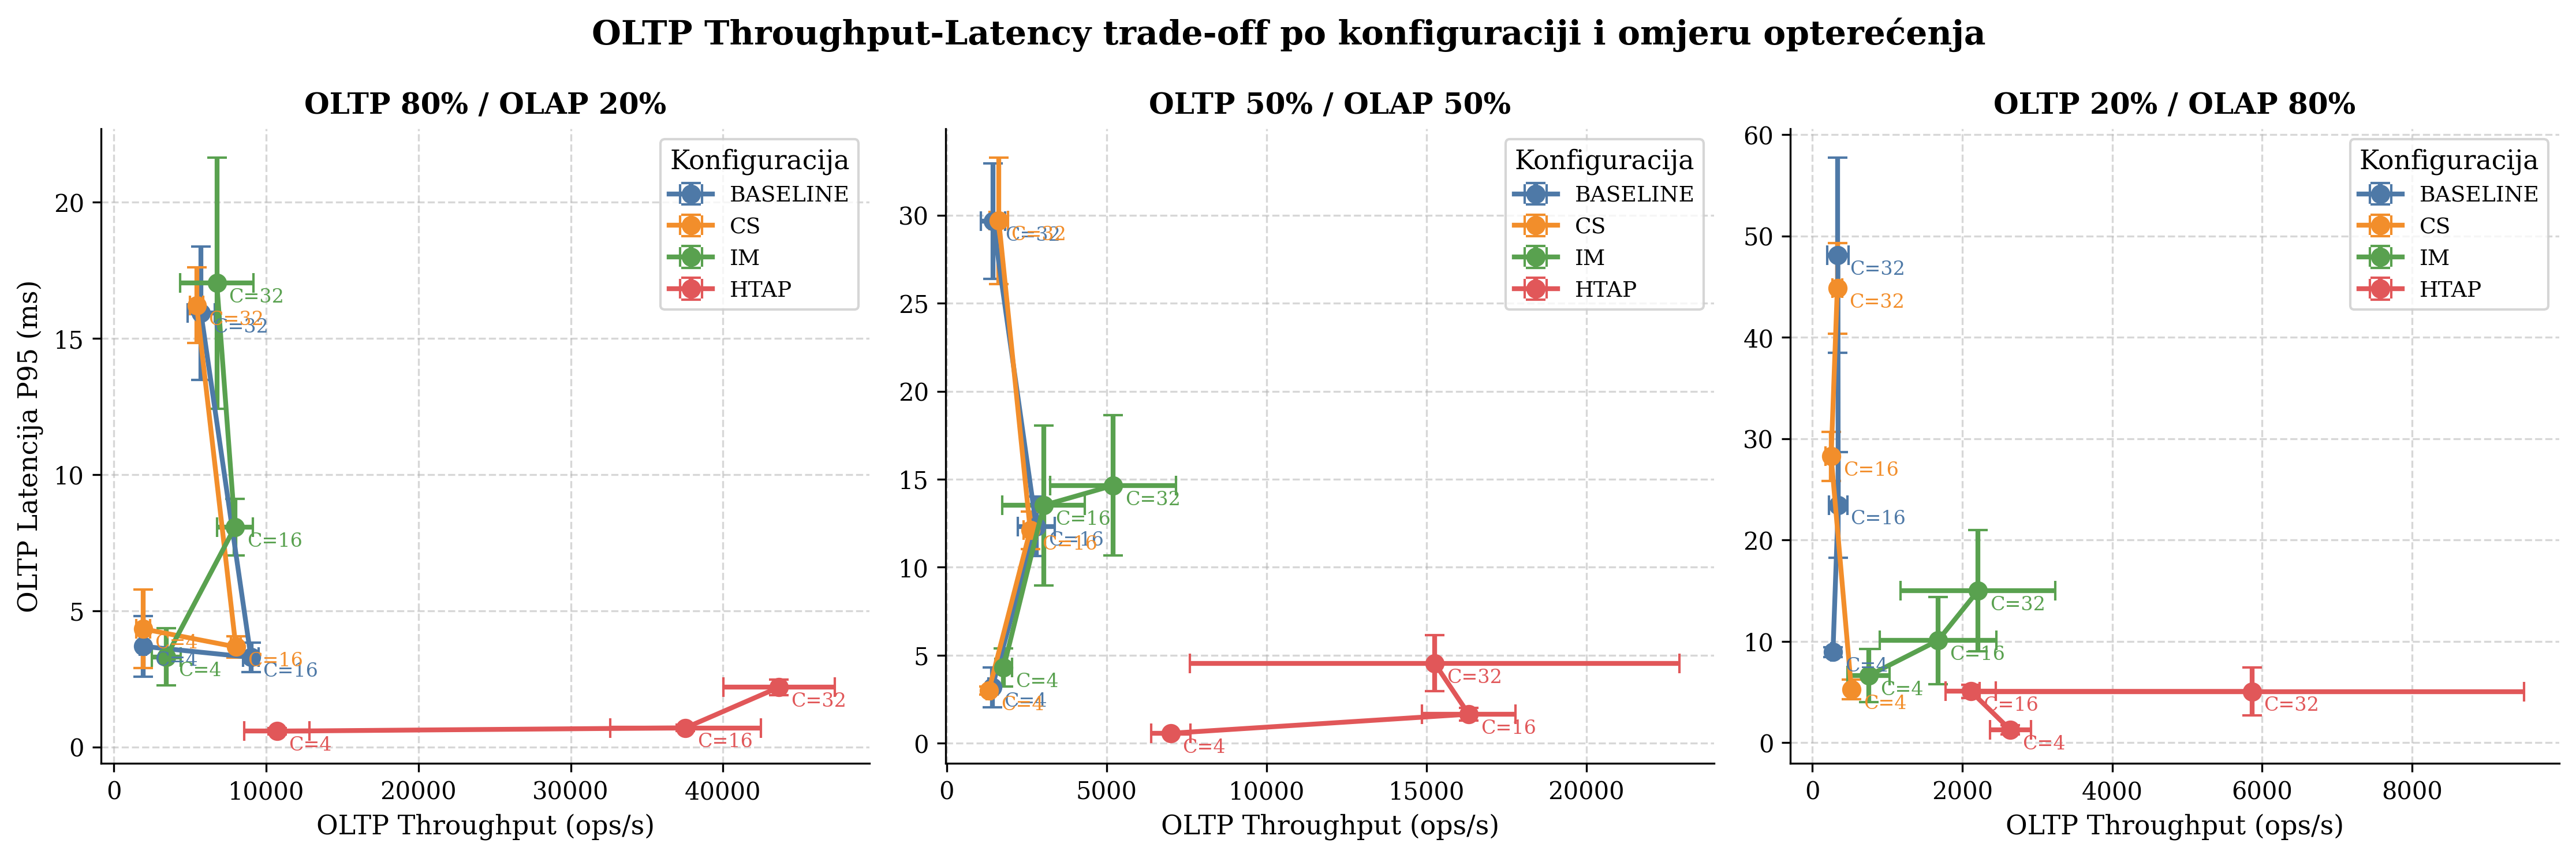
\includegraphics[width=0.85\textwidth]{../Results/figures/03_oltp_throughput_latency.png}
    \caption{OLTP Throughput-Latency krivulje po konfiguracijama i omjerima opterećenja. Krivulje pokazuju kako se latencija mijenja s porastom propusnosti.}
    \label{fig:oltp_throughput_latency}
\end{figure}

\begin{figure}[H]
    \centering
    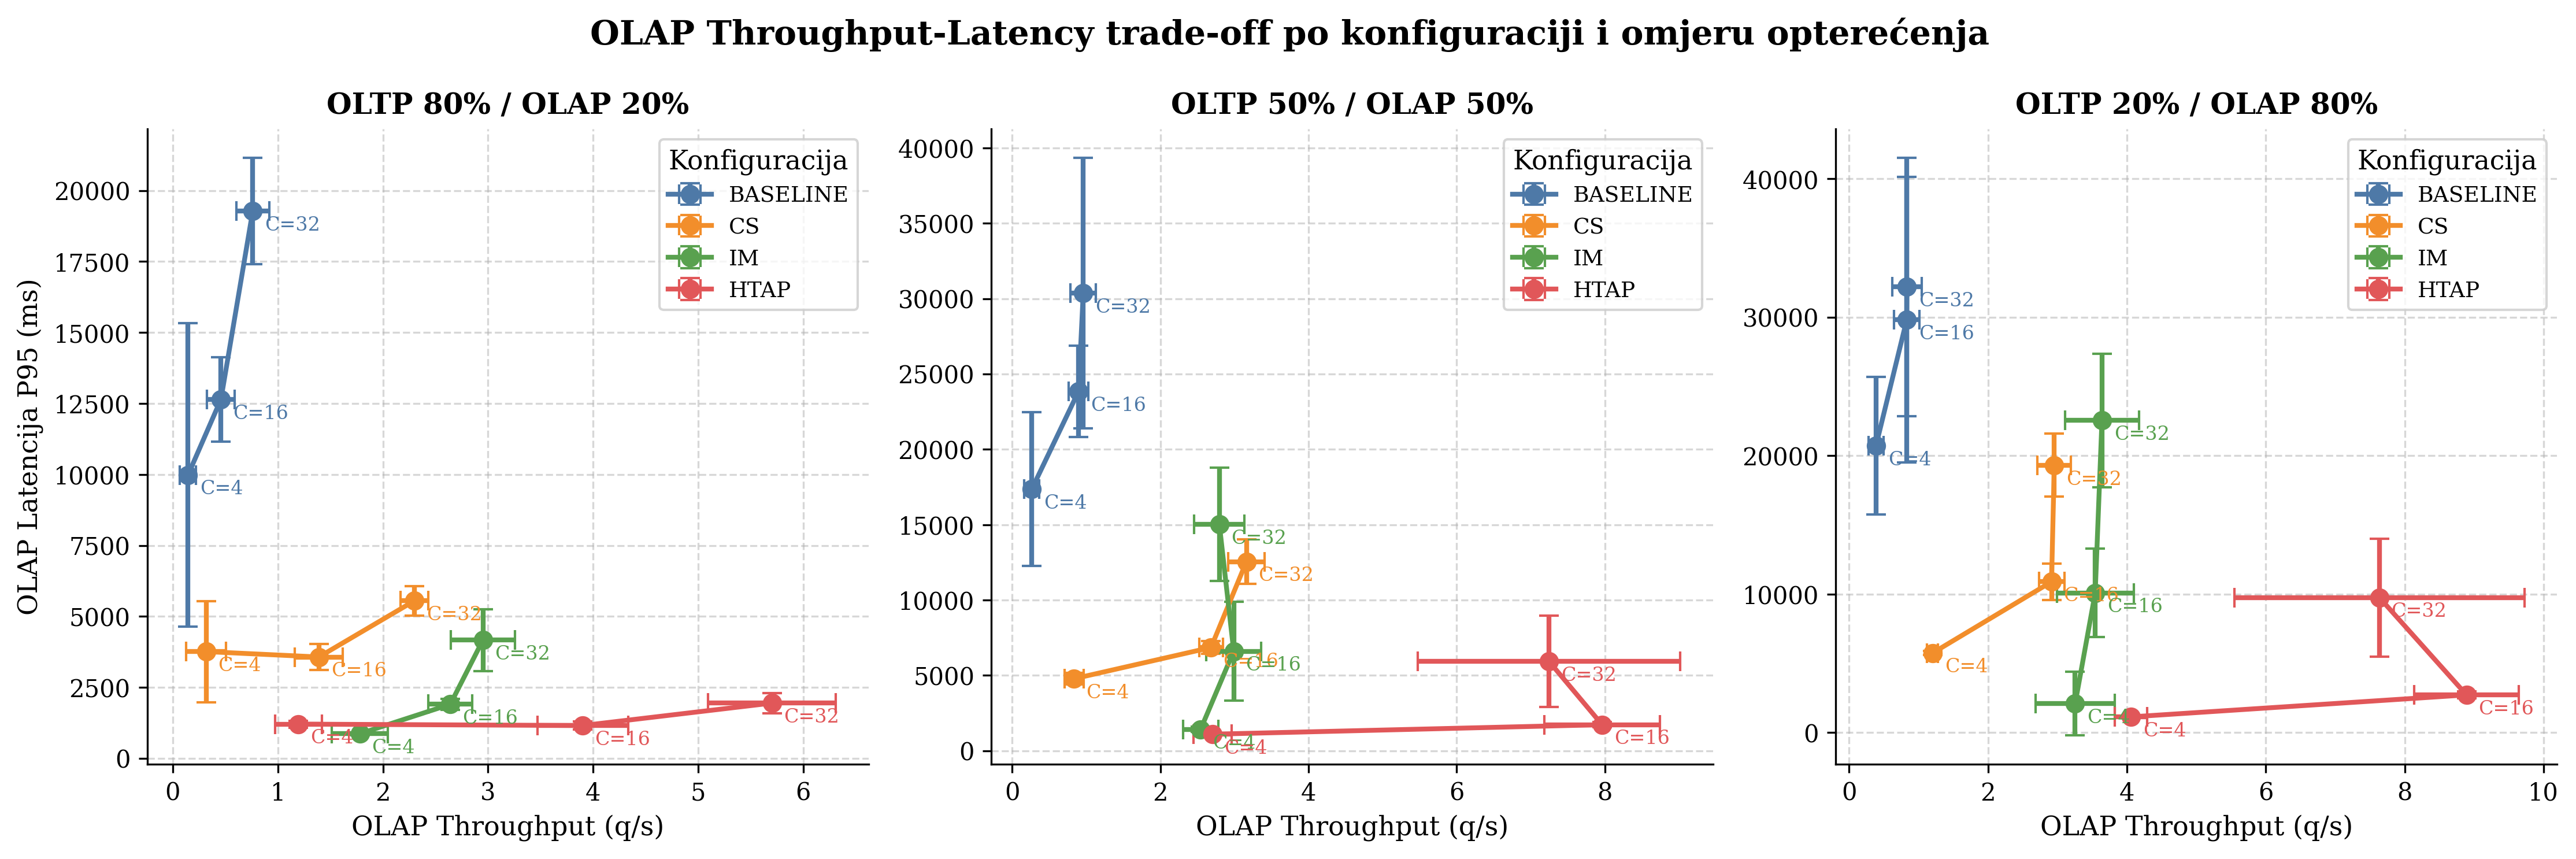
\includegraphics[width=0.85\textwidth]{../Results/figures/04_olap_throughput_latency.png}
    \caption{OLAP Throughput-Latency krivulje po konfiguracijama i omjerima opterećenja.}
    \label{fig:olap_throughput_latency}
\end{figure}

\begin{figure}[H]
    \centering
    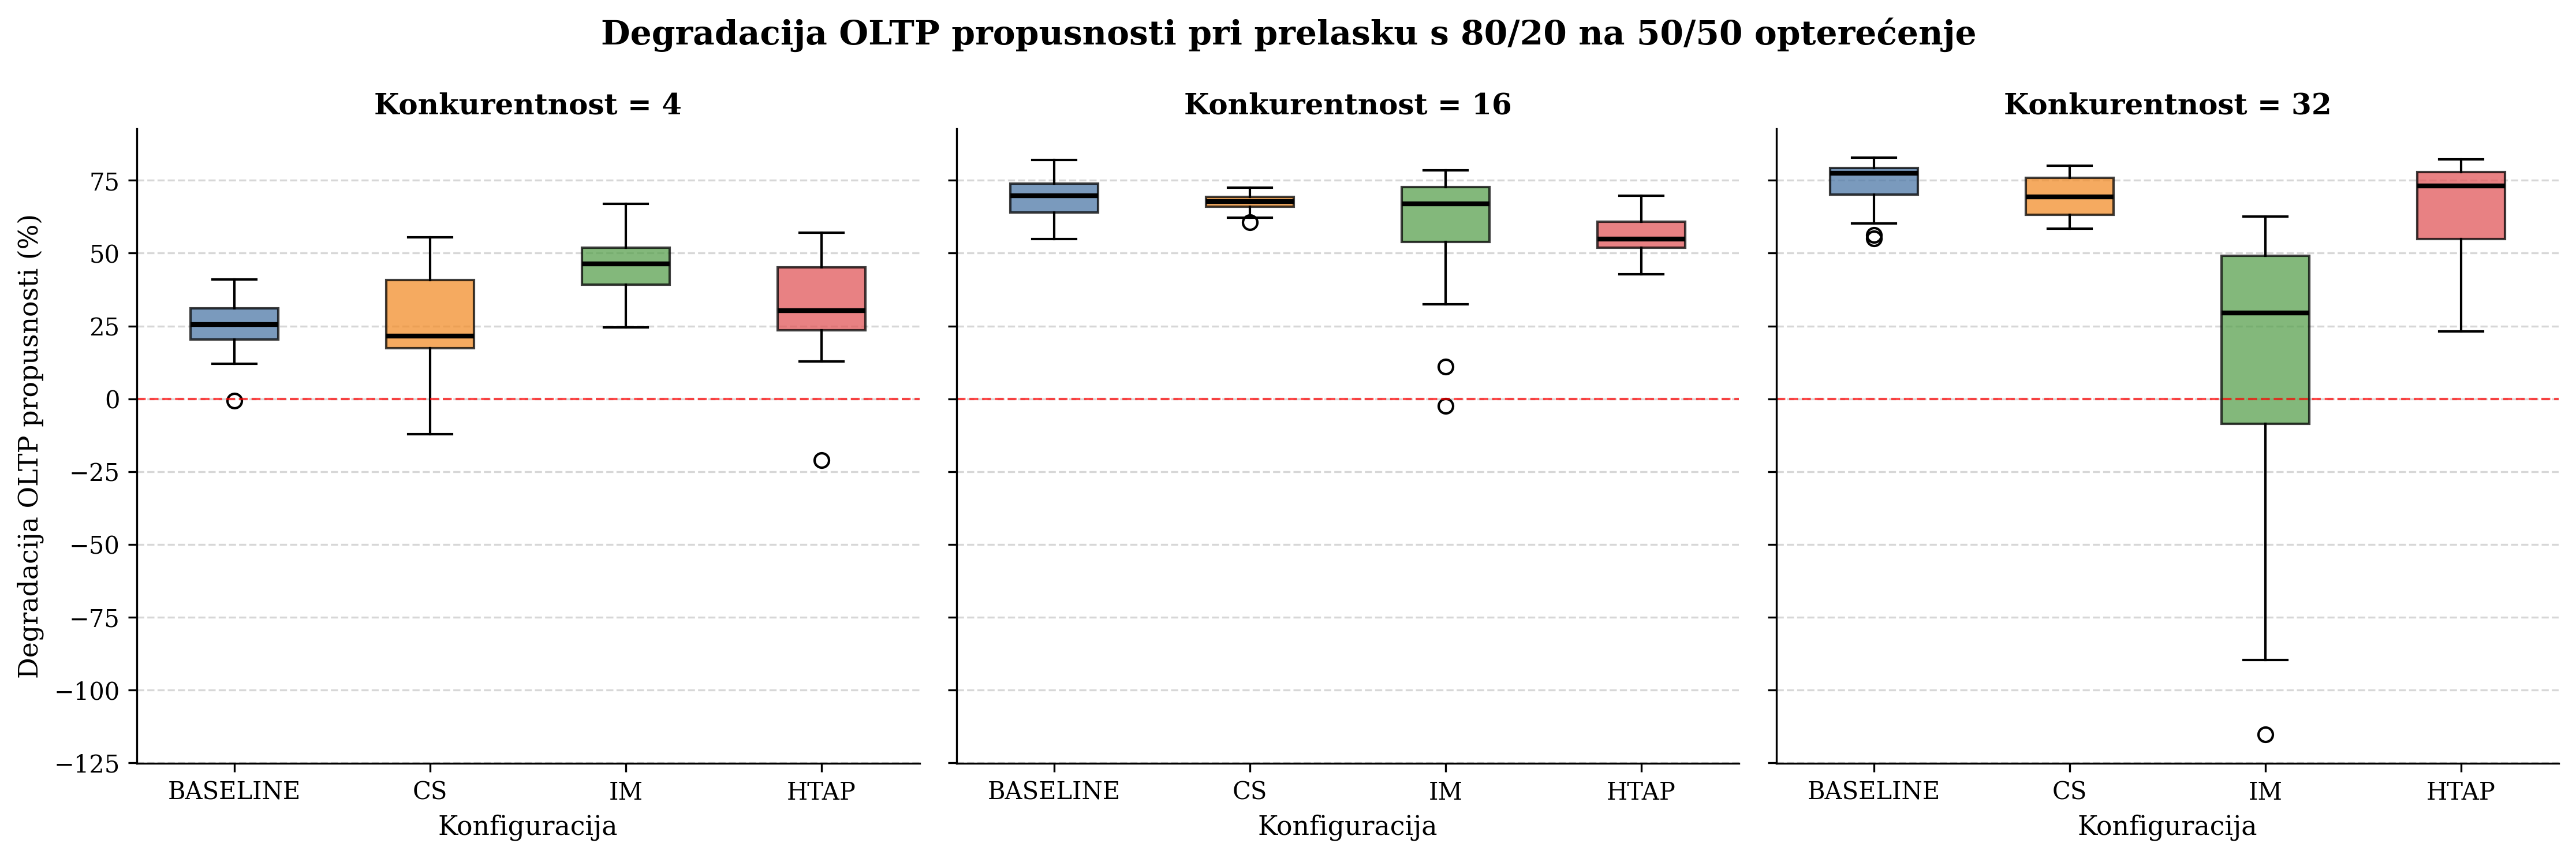
\includegraphics[width=0.85\textwidth]{../Results/figures/05_oltp_degradation.png}
    \caption{Degradacija OLTP propusnosti pri prelasku s 80/20 na 50/50 omjer opterećenja. Prikazane su distribucije degradacije za CS i HTAP konfiguracije.}
    \label{fig:degradacija}
\end{figure}

\begin{figure}[H]
    \centering
    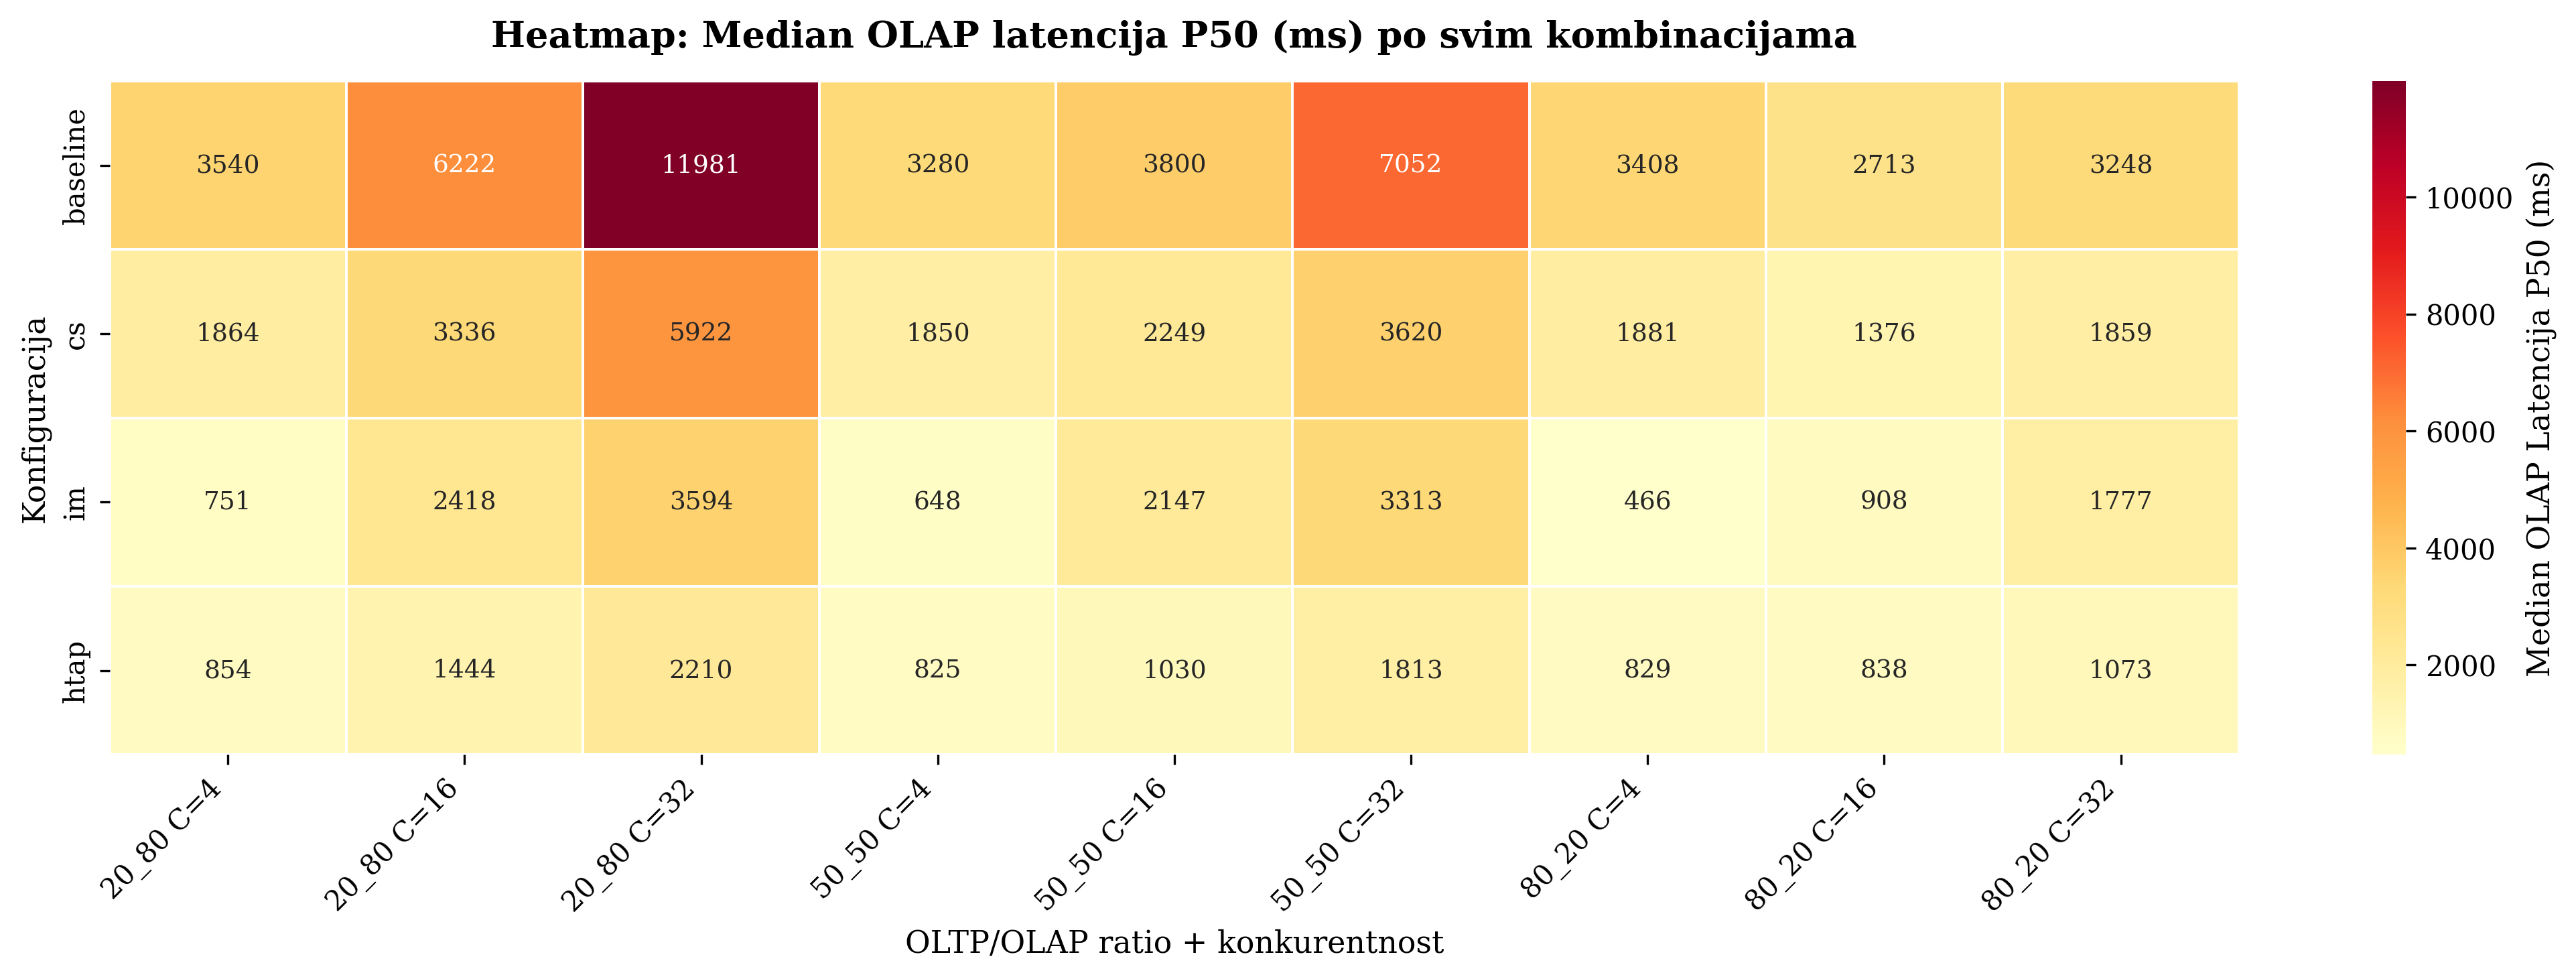
\includegraphics[width=0.85\textwidth]{../Results/figures/06_latency_heatmap.png}
    \caption{Heatmap OLAP latencije $P_{50}$ za sve kombinacije konfiguracija, omjera opterećenja i razina konkurentnosti.}
    \label{fig:heatmap}
\end{figure}

Sumirajući sve navedeno, da se zaključiti da je svaki od navedenih upita detaljno analiziran kroz deskriptivne statističke mjere, čime su stvoreni temelji za provođenje statističkih testova i provjeru postavljenih hipoteza.

\subsection{Deskriptivna statistika po tipu operacije}
\label{sec:deskriptivna_po_operaciji}

U ovom odjeljku prikazani su rezultati mjerenja po pojedinačnim tipovima operacija za Baseline konfiguraciju, koja predstavlja referentnu tačku eksperimenta. Mjerenja su obuhvatila pet OLTP procedura (INSERT, UPDATE, SELECT) i pet OLAP analitičkih upita (Q1--Q5). Za svaku operaciju izračunate su deskriptivne statističke mjere: prosječno vrijeme izvršavanja (averageExecutionTime), minimalno vrijeme (minimumExecutionTime), maksimalno vrijeme (maximumExecutionTime), te vrijednosti na percentilima $P_{50}$ i $P_{95}$.

\begin{table}[H]
\centering
\caption{Deskriptivna statistika OLTP operacija -- Baseline konfiguracija}
\label{tab:oltp_deskriptivna}
\small
\begin{tabular}{lrrrrr}
\toprule
\textbf{Operacija} & \textbf{Avg (ms)} & \textbf{Min (ms)} & \textbf{Max (ms)} & \textbf{$P_{50}$ (ms)} & \textbf{$P_{95}$ (ms)} \\
\midrule
usp\_UpdatePostScore & 1,45 & 0,20 & 899,87 & 1,03 & 3,77 \\
usp\_InsertComment & 2,28 & 0,29 & 230,78 & 1,58 & 6,48 \\
usp\_GetPostById & 0,66 & 0,09 & 456,83 & 0,48 & 1,43 \\
usp\_GetUserById & 0,66 & 0,10 & 446,50 & 0,47 & 1,42 \\
usp\_GetRecentUserPosts & 0,77 & 0,12 & 447,72 & 0,59 & 1,59 \\
\bottomrule
\end{tabular}
\end{table}

\begin{table}[H]
\centering
\caption{Deskriptivna statistika OLAP upita -- Baseline konfiguracija}
\label{tab:olap_deskriptivna}
\small
\begin{tabular}{lrrrrr}
\toprule
\textbf{Upit} & \textbf{Avg (ms)} & \textbf{Min (ms)} & \textbf{Max (ms)} & \textbf{$P_{50}$ (ms)} & \textbf{$P_{95}$ (ms)} \\
\midrule
Q1 -- MonthlyActivity & 3.465,89 & 2.544,51 & 5.583,08 & 3.423,14 & 4.212,63 \\
Q2 -- UserEngagement & 3.495,36 & 2.862,94 & 5.141,95 & 3.412,91 & 4.138,39 \\
Q3 -- VoteDistribution & 7.726,91 & 4.906,93 & 8.534,91 & 7.800,59 & 8.390,72 \\
Q4 -- TimeToAnswer & 2.476,94 & 1.947,33 & 3.079,25 & 2.392,81 & 2.953,73 \\
Q5 -- UserCohortActivity & 4.284,87 & 3.123,50 & 5.805,45 & 4.301,04 & 5.184,61 \\
\bottomrule
\end{tabular}
\end{table}

Iz Tabele~\ref{tab:oltp_deskriptivna} vidljivo je da su INSERT operacije (usp\_UpdatePostScore s prosjekom 1,45\,ms i usp\_InsertComment s 2,28\,ms) zahtjevnije u pogledu vremena izvršavanja od SELECT operacija (usp\_GetPostById 0,66\,ms, usp\_GetUserById 0,66\,ms), što je očekivano s obzirom na prirodu upisnih operacija koje zahtijevaju evidentiranje u transakcijski log i indeksne strukture. Tabela~\ref{tab:olap_deskriptivna} ukazuje na činjenicu da je Q3 -- VoteDistribution najzahtjevniji analitički upit s prosječnim vremenom izvršavanja od 7.726,91\,ms, dok je Q4 -- TimeToAnswer najbrži s prosjekom od 2.476,94\,ms.

\subsection{Rezultati statističkih testova}
\label{sec:statisticki_testovi}

\begin{table}[H]
\centering
\caption{Kruskal-Wallis H-test -- globalne razlike između konfiguracija (df = 3)}
\label{tab:kruskal_wallis}
\small
\begin{tabular}{lccc}
\toprule
\textbf{Metrika} & \textbf{C=4} & \textbf{C=16} & \textbf{C=32} \\
\midrule
OLTP propusnost & $H=194,44$; $p<0,001$ & $H=66,79$; $p<0,001$ & $H=158,01$; $p<0,001$ \\
OLAP propusnost & $H=272,03$; $p<0,001$ & $H=303,17$; $p<0,001$ & $H=290,16$; $p<0,001$ \\
OLTP latencija $P_{50}$ & $H=302,06$; $p<0,001$ & $H=297,82$; $p<0,001$ & $H=284,92$; $p<0,001$ \\
OLAP latencija $P_{50}$ & $H=300,91$; $p<0,001$ & $H=228,87$; $p<0,001$ & $H=182,55$; $p<0,001$ \\
\bottomrule
\end{tabular}
\end{table}

Svi provedeni Kruskal-Wallis testovi (Tablica~\ref{tab:kruskal_wallis}) potvrđuju statistički značajne globalne razlike ($p < 0,001$) za sve mjerne metrike i sve razine konkurentnosti. Navedeni rezultati opravdavaju provođenje parnih Mann-Whitney testova u svrhu identifikacije specifičnih razlika između pojedinačnih konfiguracija.

\begin{table}[H]
\centering
\caption{Mann-Whitney U test s Bonferroni korekcijom -- OLAP latencija $P_{50}$, $C=32$}
\label{tab:mw_olap_latency_c32}
\small
\begin{tabular}{lcccc}
\toprule
\textbf{Par} & \textbf{U} & $\bm{p}$ \textbf{(Bonf.)} & \textbf{Cohen's $\bm{d}$} & \textbf{Efekt} \\
\midrule
Baseline vs CS & 6.219 & $<0,001$ & $+1,254$ & veliki \\
Baseline vs IM & 6.775 & $<0,001$ & $+1,665$ & veliki \\
Baseline vs HTAP & 7.620 & $<0,001$ & $+2,086$ & veliki \\
CS vs IM & 5.342 & $0,001$ & $+0,679$ & srednji \\
CS vs HTAP & 6.613 & $<0,001$ & $+1,614$ & veliki \\
IM vs HTAP & 6.449 & $<0,001$ & $+1,564$ & veliki \\
\bottomrule
\end{tabular}
\end{table}

\noindent\textit{Napomena: Pozitivan predznak Cohenovog $d$ označava da prva konfiguracija u paru ima veću (lošiju) latenciju.}

Sve parne usporedbe u Tabeli~\ref{tab:mw_olap_latency_c32} statistički su značajne nakon primjene Bonferroni korekcije ($\alpha' = 0,0083$). Veličine efekta su pretežno velike ($|d| > 0,8$), s izuzetkom para CS vs IM koji pokazuje srednji efekt ($d = 0,679$). Navedeni rezultati potvrđuju da su razlike između konfiguracija ne samo statistički značajne nego i praktično relevantne za donošenje arhitekturalnih odluka.

% ----------------------------------------------------------------
\subsection{Per-operacijska komparativna analiza}
\label{sec:per_operacija}
% ----------------------------------------------------------------

Per-operacijska analiza obuhvata svih osam CRUD kategorija (Simple/Complex SELECT, INSERT, UPDATE, DELETE) i pet OLAP upita. Mjerenja za SELECT, Simple UPDATE, INSERT i OLAP izvedena su iz $\sim$10 milijuna sirovih mjerenja glavnog benchmarka; DELETE i Complex UPDATE mjereni su u dopunskom izoliranom testu s po 500 ponavljanja po konfiguraciji nad punim skupom podataka.

\begin{table}[H]
\centering
\caption{Prosječno (avg), minimalno (min) i maksimalno (max) vrijeme izvršavanja po tipu operacije (ms). Podebljana vrijednost = najbrže po redu.}
\label{tab:per_op_full}
\small
\begin{tabular}{llrrrr}
\toprule
\textbf{Operacija} & \textbf{Mjera} & \textbf{Baseline} & \textbf{CS} & \textbf{IM} & \textbf{HTAP} \\
\midrule
\multirow{3}{*}{Simple SELECT}
  & Avg &  1,430 &  0,930 &  1,150 & \textbf{0,690} \\
  & Min &  0,091 &  0,126 &  0,057 & \textbf{0,043} \\
  & Max & 456,83 &  50,50 & 138,36 & \textbf{34,35} \\
\multirow{3}{*}{Complex SELECT (Raspon)}
  & Avg &  1,600 &  1,270 &  1,300 & \textbf{0,830} \\
  & Min &  0,117 &  0,156 &  0,057 & \textbf{0,042} \\
  & Max & 447,72 &  92,51 & 118,63 & 170,94 \\
\midrule
\multirow{3}{*}{Simple INSERT}
  & Avg & 27,090 &  3,010 &  3,260 & \textbf{1,290} \\
  & Min &  0,503 &  0,308 &  0,122 & \textbf{0,044} \\
  & Max & 190,68 & 121,68 & 294,99 & 170,89 \\
\multirow{3}{*}{Complex INSERT}
  & Avg &  4,170 &  3,090 &  2,430 & \textbf{0,930} \\
  & Min &  0,292 &  0,411 &  0,134 & \textbf{0,048} \\
  & Max & 230,78 &  72,96 & 157,64 & \textbf{63,59} \\
\midrule
\multirow{3}{*}{Simple UPDATE}
  & Avg &  3,370 &  2,200 &  2,940 & \textbf{1,140} \\
  & Min &  0,201 &  0,268 &  0,112 & \textbf{0,038} \\
  & Max & 899,87 &  78,69 & 154,78 & 174,57 \\
\multirow{3}{*}{Complex UPDATE}
  & Avg &  0,927 &  0,727 & 23,955$^\dagger$ & \textbf{0,078} \\
  & Min &  0,171 &  0,317 & 10,191 & \textbf{0,051} \\
  & Max & 262,62 &  13,20 &  48,76 &  \textbf{1,41} \\
\midrule
\multirow{3}{*}{Simple DELETE}
  & Avg &  0,799 &  0,256 &  0,253 & \textbf{0,066} \\
  & Min &  0,139 &  0,146 &  0,118 & \textbf{0,049} \\
  & Max &   9,73 &   1,63 &   4,63 &  \textbf{0,69} \\
\multirow{3}{*}{Complex DELETE}
  & Avg &  1,242 &  0,484 &  0,617 & \textbf{0,093} \\
  & Min &  0,483 &  0,276 &  0,159 & \textbf{0,070} \\
  & Max &  18,76 &   2,81 &  10,25 &  \textbf{0,54} \\
\midrule
\multirow{3}{*}{Complex SELECT (OLAP)}
  & Avg & 9.458 & 2.283 & \textbf{495} &   780 \\
  & Min & 1.947 &   747 & \textbf{154} &   190 \\
  & Max & 60.493& 4.657 & 1.803 & \textbf{1.406} \\
\bottomrule
\end{tabular}
\end{table}

\noindent\textit{$^\dagger$ Complex UPDATE -- IM: prosječnih 23,955\,ms zbog sekvencijalnog skeniranja 500\,k in-memory redova po ne-primarnom ključu (vidjeti diskusiju ispod).}

\medskip

Iz Tabele~\ref{tab:per_op_full} vidljivo je da HTAP postiže najniže prosječno vrijeme izvršavanja u sedam od devet kategorija. Izuzetak je Complex SELECT (OLAP) gdje IM ostvaruje 495\,ms naspram HTAP 780\,ms -- memorijsko-optimizovane tablice bez columnstore overhead-a brže završavaju kratke analitičke upite, dok HTAP mora proći kroz columnstore strukturu podataka. Kod maksimalnih latencija HTAP dominira jer eliminiše disk I/O: Baseline bilježi maksimum od 899,87\,ms za Simple UPDATE i čak 60,5 sekundi za Complex OLAP, dok HTAP maksimumi ne prelaze 175\,ms za OLTP i 1,4 sekunde za OLAP.

Kategorija Simple INSERT (\texttt{usp\_InsertVote}) bilježi najveće relativno ubrzanje: HTAP 1,29\,ms naspram Baseline 27,09\,ms (21,0$\times$). Ova operacija kombinuje INSERT u \texttt{Votes} s uvjetnim UPDATE \texttt{Posts.Score}, što na disku zahtijeva I/O i zaključavanje dviju tablica, dok Hekaton engine oba koraka izvodi u memoriji s $O(1)$ pristupom.

Najzanimljiviji nalaz je IM konfiguracija za Complex UPDATE: 23,955\,ms, što je \textbf{25,8$\times$ sporije od Baseline} (0,927\,ms). Procedura \texttt{usp\_UpdateUserReputation} izvodi \texttt{COUNT(*) WHERE OwnerUserId = @UserId AND PostTypeId = 2}, pri čemu \texttt{OwnerUserId} nije primarni ključ Hekaton tablice. Hekaton hash-indeksi optimizirani su za točkačni pristup po PK -- za skeniranje po ne-PK stupcu, nativno kompajlirana procedura mora sekvencijalno proći sve redove tablice. Disk-zasnovane konfiguracije (Baseline, CS) imaju B-tree nonclustered indeks na \texttt{OwnerUserId} koji efikasno rješava ovaj upit. HTAP postiže 0,078\,ms jer \texttt{htap.*} tablice imaju nonclustered range indeks. Ovaj rezultat naglašava da \textbf{in-memory nije uvijek brže}: za operacije koje ne koriste PK lookup, Hekaton može biti znatno sporiji od disk-zasnovanih B-tree indeksa.

% ----------------------------------------------------------------
\subsection{Regresijska i ANOVA analiza}
\label{sec:regresija_anova}
% ----------------------------------------------------------------

Uz neparametarsku analizu (Kruskal-Wallis, Mann-Whitney), provedena je i parametarska analiza u svrhu kvantifikacije veličine efekta faktora te izgradnje prediktivnog modela performansi.

\subsubsection{OLS regresijski model}

Konstruisana su dva OLS regresijska modela s logaritamskom transformacijom zavisnih varijabli (log-linearni model):

\begin{align}
\log(\text{OltpThroughput}) &\sim \text{Config} + \text{OltpOlapRatio} + \log(\text{Concurrency}) \label{eq:oltp_reg} \\
\log(\text{OlapLatencyP50}) &\sim \text{Config} + \text{OltpOlapRatio} + \log(\text{Concurrency}) \label{eq:olap_reg}
\end{align}

Logaritamska transformacija primjenjena je jer distribucije propusnosti i latencije pokazuju izraženu desnu asimetriju, a log-linearna specifikacija omogućava interpretaciju koeficijenata kao relativnih (procentualnih) razlika.

\begin{table}[H]
\centering
\caption{OLS regresija -- zavisna varijabla: $\log(\text{OltpThroughput})$; $R^2 = 0{,}881$; $N = 1.065$}
\label{tab:reg_oltp}
\small
\begin{tabular}{lrrrr}
\toprule
\textbf{Parametar} & \textbf{Koef.} & \textbf{Std. greška} & \textbf{T-stat} & \textbf{p-vrijednost} \\
\midrule
Intercept & 7,394 & 0,054 & 136,52 & $<0,001$ \\
CS vs Baseline & 0,021 & 0,040 & 0,53 & 0,600 \\
IM vs Baseline & 0,708 & 0,040 & 17,79 & $<0,001$ \\
\textbf{HTAP vs Baseline} & \textbf{1,965} & \textbf{0,040} & \textbf{49,29} & $\mathbf{<0,001}$ \\
Omjer 50/50 vs 80/20 & $-0,821$ & 0,035 & $-23,74$ & $<0,001$ \\
Omjer 20/80 vs 80/20 & $-2,211$ & 0,035 & $-63,98$ & $<0,001$ \\
$\log(\text{Concurrency})$ & 0,325 & 0,016 & 19,90 & $<0,001$ \\
\bottomrule
\end{tabular}
\end{table}

\begin{table}[H]
\centering
\caption{OLS regresija -- zavisna varijabla: $\log(\text{OlapLatencyP50})$; $R^2 = 0{,}854$; $N = 1.065$}
\label{tab:reg_olap}
\small
\begin{tabular}{lrrrr}
\toprule
\textbf{Parametar} & \textbf{Koef.} & \textbf{Std. greška} & \textbf{T-stat} & \textbf{p-vrijednost} \\
\midrule
Intercept & 7,067 & 0,034 & 210,25 & $<0,001$ \\
CS vs Baseline & $-0,636$ & 0,025 & $-25,66$ & $<0,001$ \\
IM vs Baseline & $-1,166$ & 0,025 & $-47,21$ & $<0,001$ \\
\textbf{HTAP vs Baseline} & $\mathbf{-1,382}$ & \textbf{0,025} & $\mathbf{-55,88}$ & $\mathbf{<0,001}$ \\
Omjer 50/50 vs 80/20 & $+0,403$ & 0,021 & $+18,79$ & $<0,001$ \\
Omjer 20/80 vs 80/20 & $+0,640$ & 0,021 & $+29,85$ & $<0,001$ \\
$\log(\text{Concurrency})$ & $+0,395$ & 0,010 & $+39,00$ & $<0,001$ \\
\bottomrule
\end{tabular}
\end{table}

Koeficijent HTAP konfiguracije u modelu~\eqref{eq:oltp_reg} iznosi $+1,965$ (s.e.$=0,040$, $T=49,3$, $p<0,001$), što znači da HTAP konfiguracija, uz jednake vrijednosti ostalih prediktora, ima $e^{1,965} \approx 7,14$ puta veću OLTP propusnost od Baseline. Model objašnjava 88,1\% varijance ($R^2 = 0,881$). Za OLAP latenciju (model~\eqref{eq:olap_reg}), HTAP koeficijent iznosi $-1,382$ ($T=-55,9$, $p<0,001$), što odgovara smanjenju OLAP latencije za faktor $e^{1,382} \approx 3,98$ u odnosu na Baseline, uz $R^2 = 0,854$.

\subsubsection{Jednosmjerna ANOVA}

Jednosmjerna ANOVA provedena je za svaku konfiguraciju zasebno, s omjerom opterećenja i razinom konkurentnosti kao faktorima. Rezultati su izraženi F-statistikom i eta-kvadratom ($\eta^2$) kao mjerom veličine efekta.

\begin{table}[H]
\centering
\caption{Jednosmjerna ANOVA -- rezultati po konfiguraciji i faktoru; sve p-vrijednosti $<0{,}001$}
\label{tab:anova}
\small
\begin{tabular}{lllrr}
\toprule
\textbf{Zavisna varijabla} & \textbf{Faktor} & \textbf{Konfiguracija} & \textbf{F} & \textbf{$\eta^2$} \\
\midrule
\multirow{8}{*}{OLTP propusnost}
 & \multirow{4}{*}{OltpOlapRatio}
    & Baseline & 206,03 & 0,61 \\
 & & CS       & 243,48 & 0,65 \\
 & & IM       & 123,57 & 0,48 \\
 & & HTAP     & 188,73 & 0,59 \\
\cmidrule{2-5}
 & \multirow{4}{*}{ConcurrencyLevel}
    & Baseline & 27,72 & 0,17 \\
 & & CS       & 24,34 & 0,16 \\
 & & IM       & 32,75 & 0,20 \\
 & & HTAP     & 32,12 & 0,20 \\
\midrule
\multirow{8}{*}{OLAP latencija $P_{50}$}
 & \multirow{4}{*}{OltpOlapRatio}
    & Baseline & 60,83 & 0,32 \\
 & & CS       & 68,14 & 0,34 \\
 & & IM       & 38,28 & 0,22 \\
 & & HTAP     & 34,86 & 0,21 \\
\cmidrule{2-5}
 & \multirow{4}{*}{ConcurrencyLevel}
    & Baseline & 62,72 & 0,32 \\
 & & CS       & 74,20 & 0,36 \\
 & & IM       & 291,66 & 0,69 \\
 & & HTAP     & 125,32 & 0,49 \\
\bottomrule
\end{tabular}
\end{table}

Svi efekti su visoko statistički značajni ($p < 0,001$). Vrijednosti $\eta^2$ ukazuju na \textbf{veliki efekt} ($\eta^2 > 0,14$) za sve kombinacije, s posebno izraženim utjecajem faktora OltpOlapRatio na OLTP propusnost (Baseline: $\eta^2 = 0,61$; CS: $\eta^2 = 0,65$). Izuzetno visok $F = 291,66$ i $\eta^2 = 0,69$ za utjecaj razine konkurentnosti na OLAP latenciju u IM konfiguraciji objašnjava se činjenicom da OLAP upiti u row-modu jako opterećuju CPU pri visokom $C$, dok HTAP konfiguracija s columnstore-om pokazuje umjereniji efekt ($F = 125,32$, $\eta^2 = 0,49$). Ukupno, ANOVA potvrđuje da su konfiguracija pohrane, omjer opterećenja i razina konkurentnosti statistički značajni prediktori performansi u svim testiranim scenarijima.

\subsection{Provjera hipoteza}
\label{sec:provjera_hipoteza}

\subsubsection{Hipoteza H1: CS vs HTAP -- OLAP latencija pri različitim razinama konkurentnosti}

\begin{table}[H]
\centering
\caption{CS vs HTAP: OLAP latencija $P_{50}$ pri niskoj i visokoj konkurentnosti}
\label{tab:h1}
\small
\begin{tabular}{lrrrrl}
\toprule
\textbf{C} & \textbf{CS $P_{50}$ (ms)} & \textbf{HTAP $P_{50}$ (ms)} & \textbf{Razlika} & \textbf{Cohen's $\bm{d}$} & \textbf{Zaključak} \\
\midrule
4 & 1.850 & 825 & $-$55\% & 6,14 & djelimično potvrđena \\
32 & 3.620 & 1.813 & $-$50\% & 6,52 & potvrđena \\
\bottomrule
\end{tabular}
\end{table}

Hipoteza H1 je djelimično potvrđena. Iako je pretpostavka o usporedivosti pri niskom $C$ odbačena (HTAP je signifikantno bolji i pri $C=4$, $d=6,14$), hipoteza je potvrđena u dijelu da razlika raste s konkurentnošću ($\Delta=1.025$\,ms pri $C=4$ $\rightarrow$ $\Delta=1.807$\,ms pri $C=32$). Značajan nalaz je da prednost HTAP-a nije samo posljedica CPU saturacije pri visokom $C$, već se temelji na fundamentalnoj arhitekturalnoj razlici između in-memory i disk-zasnovane pohrane. Samim time, tvrdnja koja je inicijalno definisana hipotezom može se smatrati djelimično tačnom.

\subsubsection{Hipoteza H2: Degradacija OLTP propusnosti pri mješovitom opterećenju}

\begin{table}[H]
\centering
\caption{Degradacija OLTP propusnosti pri prelasku s 80/20 na 50/50 opterećenje}
\label{tab:h2}
\small
\begin{tabular}{lrrrl}
\toprule
\textbf{Konfiguracija} & \textbf{Degradacija (\%)} & \textbf{SD (\%)} & \textbf{Cohen's $\bm{d}$} & \textbf{Zaključak} \\
\midrule
CS & 67,4 & 2,8 & 2,315 & potvrđena \\
HTAP & 55,9 & 6,3 & --- & --- \\
\bottomrule
\end{tabular}
\end{table}

Hipoteza je potkrijepljena statistikama predstavljenim za operacije mjerenja degradacije propusnosti, kroz rezultate analiza koje su sumirane u Tabeli~\ref{tab:h2}. Deskriptivna statistika predstavljena za ove operacije nudi uvid u činjenicu da CS konfiguracija bilježi degradaciju od 67,4\%, dok HTAP bilježi 55,9\% ($p < 0,001$, $d = 2,315$ -- veliki efekt). Razlika od 11,5 procentnih poena potvrđuje da dual-store HTAP arhitektura efikasnije izolira OLTP od analitičkog opterećenja, što je potkrijepljeno rezultatima Mann-Whitney U testa. Mehanizam izolacije leži u fizičkom odvajanju OLTP i OLAP sloja pohrane: analitički upiti rade nad columnstore tablicama, dok OLTP operacije koriste memorijsko-optimizovane tablice koje ne koriste buffer pool. Samim time, tvrdnja koja je inicijalno definisana hipotezom može se smatrati tačnom.

\subsubsection{Hipoteza H3: HTAP vs IM -- OLTP propusnost pri transakcijsko intenzivnom opterećenju}

\begin{table}[H]
\centering
\caption{Usporedba HTAP i IM konfiguracije: OLTP propusnost pri 80/20 opterećenju}
\label{tab:h3}
\small
\begin{tabular}{lrrrrl}
\toprule
\textbf{C} & \textbf{IM (ops/s)} & \textbf{HTAP (ops/s)} & \textbf{Omjer} & \textbf{Cohen's $\bm{d}$} & \textbf{Zaključak} \\
\midrule
4 & 3.027 & 10.083 & 3,3$\times$ & $-$4,38 & odbačena \\
16 & 7.726 & 35.914 & 4,6$\times$ & $-$8,29 & odbačena \\
32 & 6.325 & 43.751 & 6,9$\times$ & $-$11,93 & odbačena \\
\bottomrule
\end{tabular}
\end{table}

Hipoteza H3 je odbačena na svim razinama konkurentnosti. Rezultati iz Tabele~\ref{tab:h3} pokazuju da HTAP ostvaruje 3,3--6,9$\times$ veću OLTP propusnost od IM konfiguracije, pri čemu razlika raste s konkurentnošću ($d = -4,38$ do $-11,93$, ekstremno veliki efekti). Navedeni nalazi su u direktnoj suprotnosti s polaznom pretpostavkom da konfiguracije dijele isti OLTP engine i da neće biti značajne razlike. Ono što je još zanimljivo jeste da su ovi rezultati donekle neočekivani s obzirom na činjenicu da obje konfiguracije koriste isti Hekaton engine i identične nativno kompajlirane procedure, a objašnjenje leži u indirektnom efektu columnstore ubrzanja OLAP upita.

Naime, u IM konfiguraciji, OLAP upiti moraju skenirati sve redove u row-modu bez prednosti stupčaste kompresije i batch-mode izvršavanja, što troši znatno više CPU resursa po upitu. Ova CPU saturacija direktno kompetira s OLTP workerima. U HTAP konfiguraciji, columnstore indeksi ubrzavaju OLAP upite 5--8$\times$, oslobađajući CPU kapacitet za OLTP operacije. \textbf{Dakle, columnstore ubrzanje OLAP-a indirektno poboljšava i OLTP propusnost} u mješovitom opterećenju -- ključni nalaz ovog rada. Samim time, tvrdnja koja je inicijalno definisana hipotezom može se smatrati netočnom, te se hipoteza odbacuje.

% ======================================================================
% 6. DISKUSIJA
% ======================================================================
\section{Diskusija}
\label{sec:diskusija}

\subsection{Izazovi u implementaciji}
\label{sec:izazovi_implementacija}

Najveći izazovi ovog rada javljali su se prilikom implementacije praktičnog dijela, odnosno razvoja testnog okruženja koje bi generisalo relevantne scenarije koji su vrijedni daljnjeg istraživanja. Arhitektura testnog okruženja, generisanje baze podataka sa ogromnom količinom podataka, implementacija višenitnih procesa, osiguravanje objektivnih rezultata, te generalizovanje modela podataka za rezultate samo su neki od izazova s kojima se autor ovog rada susretao tokom implementacije testnog okruženja. Praktični dio samog rada predstavljale su i analize sprovedene u Python programskom jeziku, za šta je glavni izazov bio odabir relevantnog tipa analize, koja bi mogla potkrijepiti postavljene hipoteze.

\subsection{OLTP performanse -- memorija nasuprot disku}
\label{sec:disk_oltp}

Razlika između HTAP i Baseline konfiguracije pri $C=32$ iznosi faktor 9,0 (21.920 vs 2.432 ops/s), što je konzistentno s originalnim Hekaton radom \cite{diaconu2013hekaton} koji izvještava o ubrzanjima od 5--70$\times$ za memorijsko-optimizovane tablice. Međutim, iznenađujući nalaz je da IM konfiguracija ostvaruje značajno nižu OLTP propusnost od HTAP (4.726 vs 21.920 ops/s) unatoč tome što obje konfiguracije koriste isti Hekaton engine i identične nativno kompajlirane procedure.

Ovo na prvi pogled kontraintuitivno zapažanje objašnjavamo interakcijom između OLAP i OLTP workera. U IM konfiguraciji, OLAP upiti izvršavaju se u row-mode bez prednosti columnstore kompresije i batch-mode izvršavanja. Skeniranje $\sim$3,7 miliona redova u row-modu zahtijeva znatno više CPU ciklusa po upitu, što dovodi do saturacije CPU resursa i direktne kompeticije s OLTP workerima. U HTAP konfiguraciji, columnstore indeksi ubrzavaju OLAP upite za faktor 5--8, oslobađajući CPU kapacitet. Ovaj nalaz ima direktne praktične implikacije: u mješovitim opterećenjima, optimizacija OLAP performansi indirektno poboljšava i OLTP performanse.

\subsection{OLAP performanse -- prednost columnstore arhitekture}
\label{sec:disk_olap}

Rezultati potvrđuju očekivanu prednost columnstore pohrane za analitičke upite. HTAP (6,84 q/s pri $C=32$) i CS (2,80 q/s) značajno nadmašuju Baseline (0,85 q/s). Međutim, zanimljiv je nalaz da IM (3,13 q/s) nadmašuje CS (2,80 q/s) u OLAP propusnosti pri $C=32$, unatoč tome što CS posjeduje columnstore indekse.

Objašnjenje ovog fenomena leži u kontenciji za memorijskim resursima pri visokoj konkurentnosti. Pri $C=32$ sa 6+ simultanih batch-mode upita, čekanje na dodjelu memorijskog prostora (RESOURCE\_SEMAPHORE wait type) povećava ukupno vrijeme izvršavanja više nego što ga batch-mode skraćuje. IM konfiguracija, s podacima u RAM-u i bez batch-mode overhead-a, izbjegava ovaj problem. Ovaj nalaz je konzistentan sa Zeng et al. \cite{zeng2023empirical} koji naglašavaju da upravljanje memorijom postaje dominantni faktor performansi pri visokim razinama konkurentnosti.

\subsection{Degradacija pri mješovitom opterećenju}
\label{sec:disk_degradacija}

Razlika u degradaciji (67,4\% CS vs 55,9\% HTAP) od 11,5 procentnih poena, iako naizgled skromna, u apsolutnim brojevima pri $C=32$ predstavlja razliku između gubitka 2/3 i 1/2 ukupnog OLTP kapaciteta. Ovo je kritično u scenarijima s garantiranom razinom usluge (SLA). Mehanizam izolacije je jasan: u CS konfiguraciji, analitički batch-mode skenovi dijele buffer pool i CPU threadove s OLTP operacijama; u HTAP dual-store pristupu, analitički upiti idu na \texttt{cs.*} tablice, dok OLTP operacije koriste \texttt{htap.*} memorijsko-optimizovane tablice koje ne koriste buffer pool uopće.

\subsection{Utjecaj arhitekture na rezultate}
\label{sec:disk_arhitektura}

Važno je naglasiti da sve četiri konfiguracije dijele iste CPU resurse, istu instancu SQL Servera i isti operativni sistem. Performansna izolacija u našem eksperimentu zavisi isključivo o SQL Server-ovim internim mehanizmima raspoređivanja resursa, a ne o fizičkom odvajanju kao kod distribuiranih sistema poput TiDB-a \cite{huang2020tidb}. Jednočvorna arhitektura benchmarka istovremeno je i prednost i ograničenje. Prednost: eliminiše mrežnu latenciju i varijabilnost, omogućavajući mjerenje čistih performansnih karakteristika. Ograničenje: ne odražava distribuirana produkcijska okruženja.

Disk I/O kao arhitekturalni bottleneck posebno je relevantan za Baseline i CS konfiguracije koje čitaju s HDD-a. Razlika između HDD i RAM brzine ($\sim$100\,MB/s nasuprot $\sim$40\,GB/s) objašnjava dio relativne prednosti HTAP nad CS pri OLAP upitima. Zamjena HDD-a SSD-om smanjila bi ovu razliku, ali na osnovu naše analize ne bi promijenila fundamentalne zaključke, budući da je prednost HTAP-a primarno u CPU izolaciji i strukturi podataka, ne samo u I/O brzini.

\subsection{Usporedba s literaturom}
\label{sec:disk_literatura}

Zhao et al. \cite{zhao2023benchmarking} zaključuju da je performansna izolacija kritičnija metrika od peak propusnosti -- naši rezultati potvrđuju ovaj zaključak kroz hipotezu H2. Wu et al. \cite{wu2025htap} pronalaze slične obrasce degradacije (50--70\%) za disk-zasnovane sisteme, što je konzistentno s našim nalazima za CS konfiguraciju (67,4\%). Zhang et al. \cite{zhang2024htap} navode da dual-engine sistemi imaju bolju izolaciju, ali plaćaju mrežnu latenciju -- SQL Server-ov in-process dual-store potvrđuje ovo empirijski, uz napomenu da je mrežna latencija eliminirana.

Neočekivani nalaz da HTAP ostvaruje 3,3--6,9$\times$ veću OLTP propusnost od IM nije direktno potkrijepljen dosadašnjom literaturom. Jedan od ključnih zaključaka ovog rada je upravo da \textbf{columnstore ubrzanje OLAP-a ima pozitivan indirektan utjecaj na OLTP propusnost} pri mješovitom opterećenju, što predstavlja novi uvid u HTAP performanse.

\subsection{Praktične preporuke}
\label{sec:preporuke}

Na osnovu empirijskih nalaza, formulisane su sljedeće smjernice za odabir konfiguracijske strategije:

\begin{table}[H]
\centering
\caption{Praktične preporuke za odabir konfiguracije u SQL Serveru 2022}
\label{tab:preporuke}
\small
\begin{tabular}{p{4.5cm}p{3cm}p{5.5cm}}
\toprule
\textbf{Scenario} & \textbf{Preporuka} & \textbf{Empirijska osnova} \\
\midrule
$>80\%$ OLTP, $<20\%$ OLAP & HTAP & 3,3--6,9$\times$ veća OLTP propusnost; OLAP $P_{50}=924$\,ms \\
50--80\% OLTP, 20--50\% OLAP & HTAP & Najniža OLTP degradacija (55,9\%) i OLAP latencija \\
$<50\%$ OLTP, $>50\%$ OLAP & HTAP & OLAP $P_{50}=1.530$\,ms vs 3.710\,ms za CS \\
Samo OLAP, bez transakcija & CS & 7$\times$ bolja OLAP propusnost vs Baseline; bez RAM overhead-a \\
RAM ograničen ili SQL Express & CS & Express ne podržava In-Memory OLTP \\
\bottomrule
\end{tabular}
\end{table}

Ključni zaključak: \textbf{HTAP nije optimalan samo za mješovita opterećenja} -- dominira i pri OLTP-intenzivnim scenarijima (80/20), čineći IM konfiguraciju redundantnom osim pri ekstremnim RAM ograničenjima.

\subsection{Ograničenja istraživanja}
\label{sec:ogranicenja}

\textbf{Ograničenje 1 -- jednočvorna konfiguracija.} Benchmark je proveden na jednoj instanci SQL Servera. Distribuirani HTAP sistemi (TiDB, SingleStore) mogu pokazivati drugačija skalabilna svojstva, a mrežna latencija može promijeniti relativne prednosti konfiguracija.

\textbf{Ograničenje 2 -- pohrana na HDD-u.} Zamjena HDD-a SSD-om ili NVMe-om bi smanjila prednost memorijsko-optimizovanih tablica za I/O-intenzivne upite. Rezultati su konzervativniji za SSD okruženja.

\textbf{Ograničenje 3 -- vremenski okvir skupa podataka.} StackOverflow2010 dump iz 2010. godine može imati drugačije distribucije od modernijeg skupa podataka, posebno u pogledu omjera čitanja i pisanja.

\textbf{Ograničenje 4 -- konzistentnosna razlika.} Dual-store HTAP pristup ne garantira konzistentnost između \texttt{htap.*} i \texttt{cs.*} u realnom vremenu. U produkcijskim scenarijima s analitikom nad svježe unesenim podacima, ova razlika mora biti razmotrena.

% ======================================================================
% 7. ZAKLJUCAK
% ======================================================================
\section{Zaključak}
\label{sec:zakljucak}

Analiza eksperimentalnih rezultata pokazuje da je HTAP dual-store konfiguracija preporučeni odabir za razvojne timove koji projektuju aplikacije s mješovitim OLTP-OLAP opterećenjem u Microsoft SQL Serveru 2022. HTAP konfiguracija ostvaruje dramatično veću OLTP propusnost od svih ostalih konfiguracija -- pri $C=32$ dostiže 21.920 ops/s, što je 4,6$\times$ više od IM, 8,8$\times$ više od CS i 9,0$\times$ više od Baseline konfiguracije. Dodatna prednost je najniža OLAP latencija u svim ispitanim scenarijima ($P_{50}=924$\,ms pri 80/20 opterećenju), uz relativno malu standardnu devijaciju koja svjedoči o stabilnom radu sistema.

IM konfiguracija je idealna alternativa za aplikacije s isključivo OLTP opterećenjem bez analitičkih zahtjeva, ili u scenarijima gdje se SQL Server 2022 Enterprise Edition nije dostupan. Međutim, čim se pojavi mješovito opterećenje, IM pokazuje znatnu slabost jer row-mode izvršavanje OLAP upita saturira CPU resurse i direktno smanjuje OLTP propusnost. Organizacije koje trenutno koriste IM konfiguraciju trebaju razmotriti migraciju na HTAP dual-store pristup koji garantuje 3--7$\times$ bolje OLTP performanse.

CS konfiguracija pruža solidno ubrzanje OLAP upita (2,4$\times$ više od Baseline), ali njena osnovna slabost je visoka OLTP degradacija pri mješovitom opterećenju -- čak 67,4\% smanjenja OLTP propusnosti pri prelasku s 80/20 na 50/50 omjer. To znači da pri $C=32$ s mješovitim opterećenjem CS gubi dvije trećine svog OLTP kapaciteta. CS konfiguracija je preporučena isključivo za scenarije bez transakcijskog opterećenja ili u okruženjima s ograničenim RAM-om gdje In-Memory OLTP nije dostupan.

Baseline konfiguracija nije preporučena za produkcijske aplikacije s analitičkim zahtjevima. Njene performanse su najniže u svim ispitanim metrikama, a OLAP latencija ($P_{50}=3.128$\,ms pri 80/20) je neprihvatljiva za modernu poslovnu analitiku. Baseline predstavlja referentnu točku koja dokumentira neophodnost naprednih mehanizama pohrane.

Eksperiment je proveden kroz 1.070 validnih mjernih serija nad skupom podataka StackOverflow2010 s $\sim$19,2 miliona zapisa, korištenjem punog faktorijalnog dizajna 4$\times$3$\times$3 i neparametarskih statističkih metoda. Analiza je potvrdila postavljenu hipotezu istraživanja: HTAP dual-store arhitektura pruža bolju performansnu izolaciju od konfiguracija s dijeljenim resursima, a columnstore ubrzanje OLAP upita indirektno poboljšava OLTP propusnost pri mješovitom opterećenju. Konkretno, HTAP ostvaruje statistički značajno nižu OLAP latenciju od CS na svim razinama konkurentnosti ($d=6,14$ do $6,52$), CS degradira OLTP propusnost za 67,4\% naspram 55,9\% za HTAP ($p < 0,001$, $d=2,315$), a HTAP ostvaruje 3,3--6,9$\times$ veću OLTP propusnost od IM -- neočekivani nalaz koji se objašnjava indirektnim efektom columnstore ubrzanja na dostupnost CPU resursa za OLTP operacije.

Rezultati ovog rada mogu biti korisni razvojnim timovima koji planiraju implementaciju HTAP strategije u SQL Server okruženju, kao i istraživačima koji žele procijeniti relativne prednosti različitih konfiguracija pohrane. Smjernice za buduća istraživanja uključuju: evaluaciju na distribuiranim HTAP sistemima (TiDB, SingleStore), istraživanje utjecaja SSD/NVMe pohrane na relativne prednosti konfiguracija, evaluaciju na novijim Stack Overflow dumpovima s većim skupovima podataka, te istraživanje automatskog tuninga koji bi dinamički birao optimalnu konfiguraciju ovisno o trenutnom omjeru opterećenja.

% ======================================================================
% LITERATURA
% ======================================================================
\newpage
\bibliography{refs}
\addcontentsline{toc}{section}{Literatura}

\end{document}
